\documentclass[9pt,t,xcolor=table]{beamer}
\usetheme{kuleuven2}
\usepackage[english]{babel}
\usepackage{amsfonts}
\usepackage{amssymb}
\useinnertheme{circles}
\usefonttheme[onlymath]{serif}	
\usepackage{mathtools}
\usepackage{amsmath}
\setbeamertemplate{footline}[body]
\usepackage{physics}
\usepackage{chemfig}
\usepackage{graphicx}
\usepackage{mdframed}
\usepackage{cancel}
\usepackage{textcomp}
\usepackage{xcolor}
\usepackage[english]{babel}
\usepackage{soul}
\usepackage{setspace}
\usepackage{fancyvrb}
\usepackage[export]{adjustbox}
\usepackage{mathtools,booktabs,amsmath,upgreek,amsfonts,amssymb,multirow,tikz}
\usepackage[utf8]{inputenc}
\usepackage{csquotes}
\usepackage[absolute, overlay]{textpos}
\usepackage[T1]{fontenc}
\usepackage{pgfplots}
\pgfplotsset{compat=1.18}
\def\Put(#1,#2)#3{\leavevmode\makebox(0,0){\put(#1,#2){#3}}}

\title{Non-valence anions of biological molecules}
\subtitle{TCCM}
%\author{Mauro Gascón Navas}
\author{Mauro Gascón \\ HPC User Day}
%\institute{Prof. Thomas Jagau}
\date{June 2, 2025}
\renewcommand\fbox{\fcolorbox{blue}{white}}

\begin{document}

% title frame
\begin{frame}[plain,noframenumbering]
	\titlepage
	\Put(155,-530){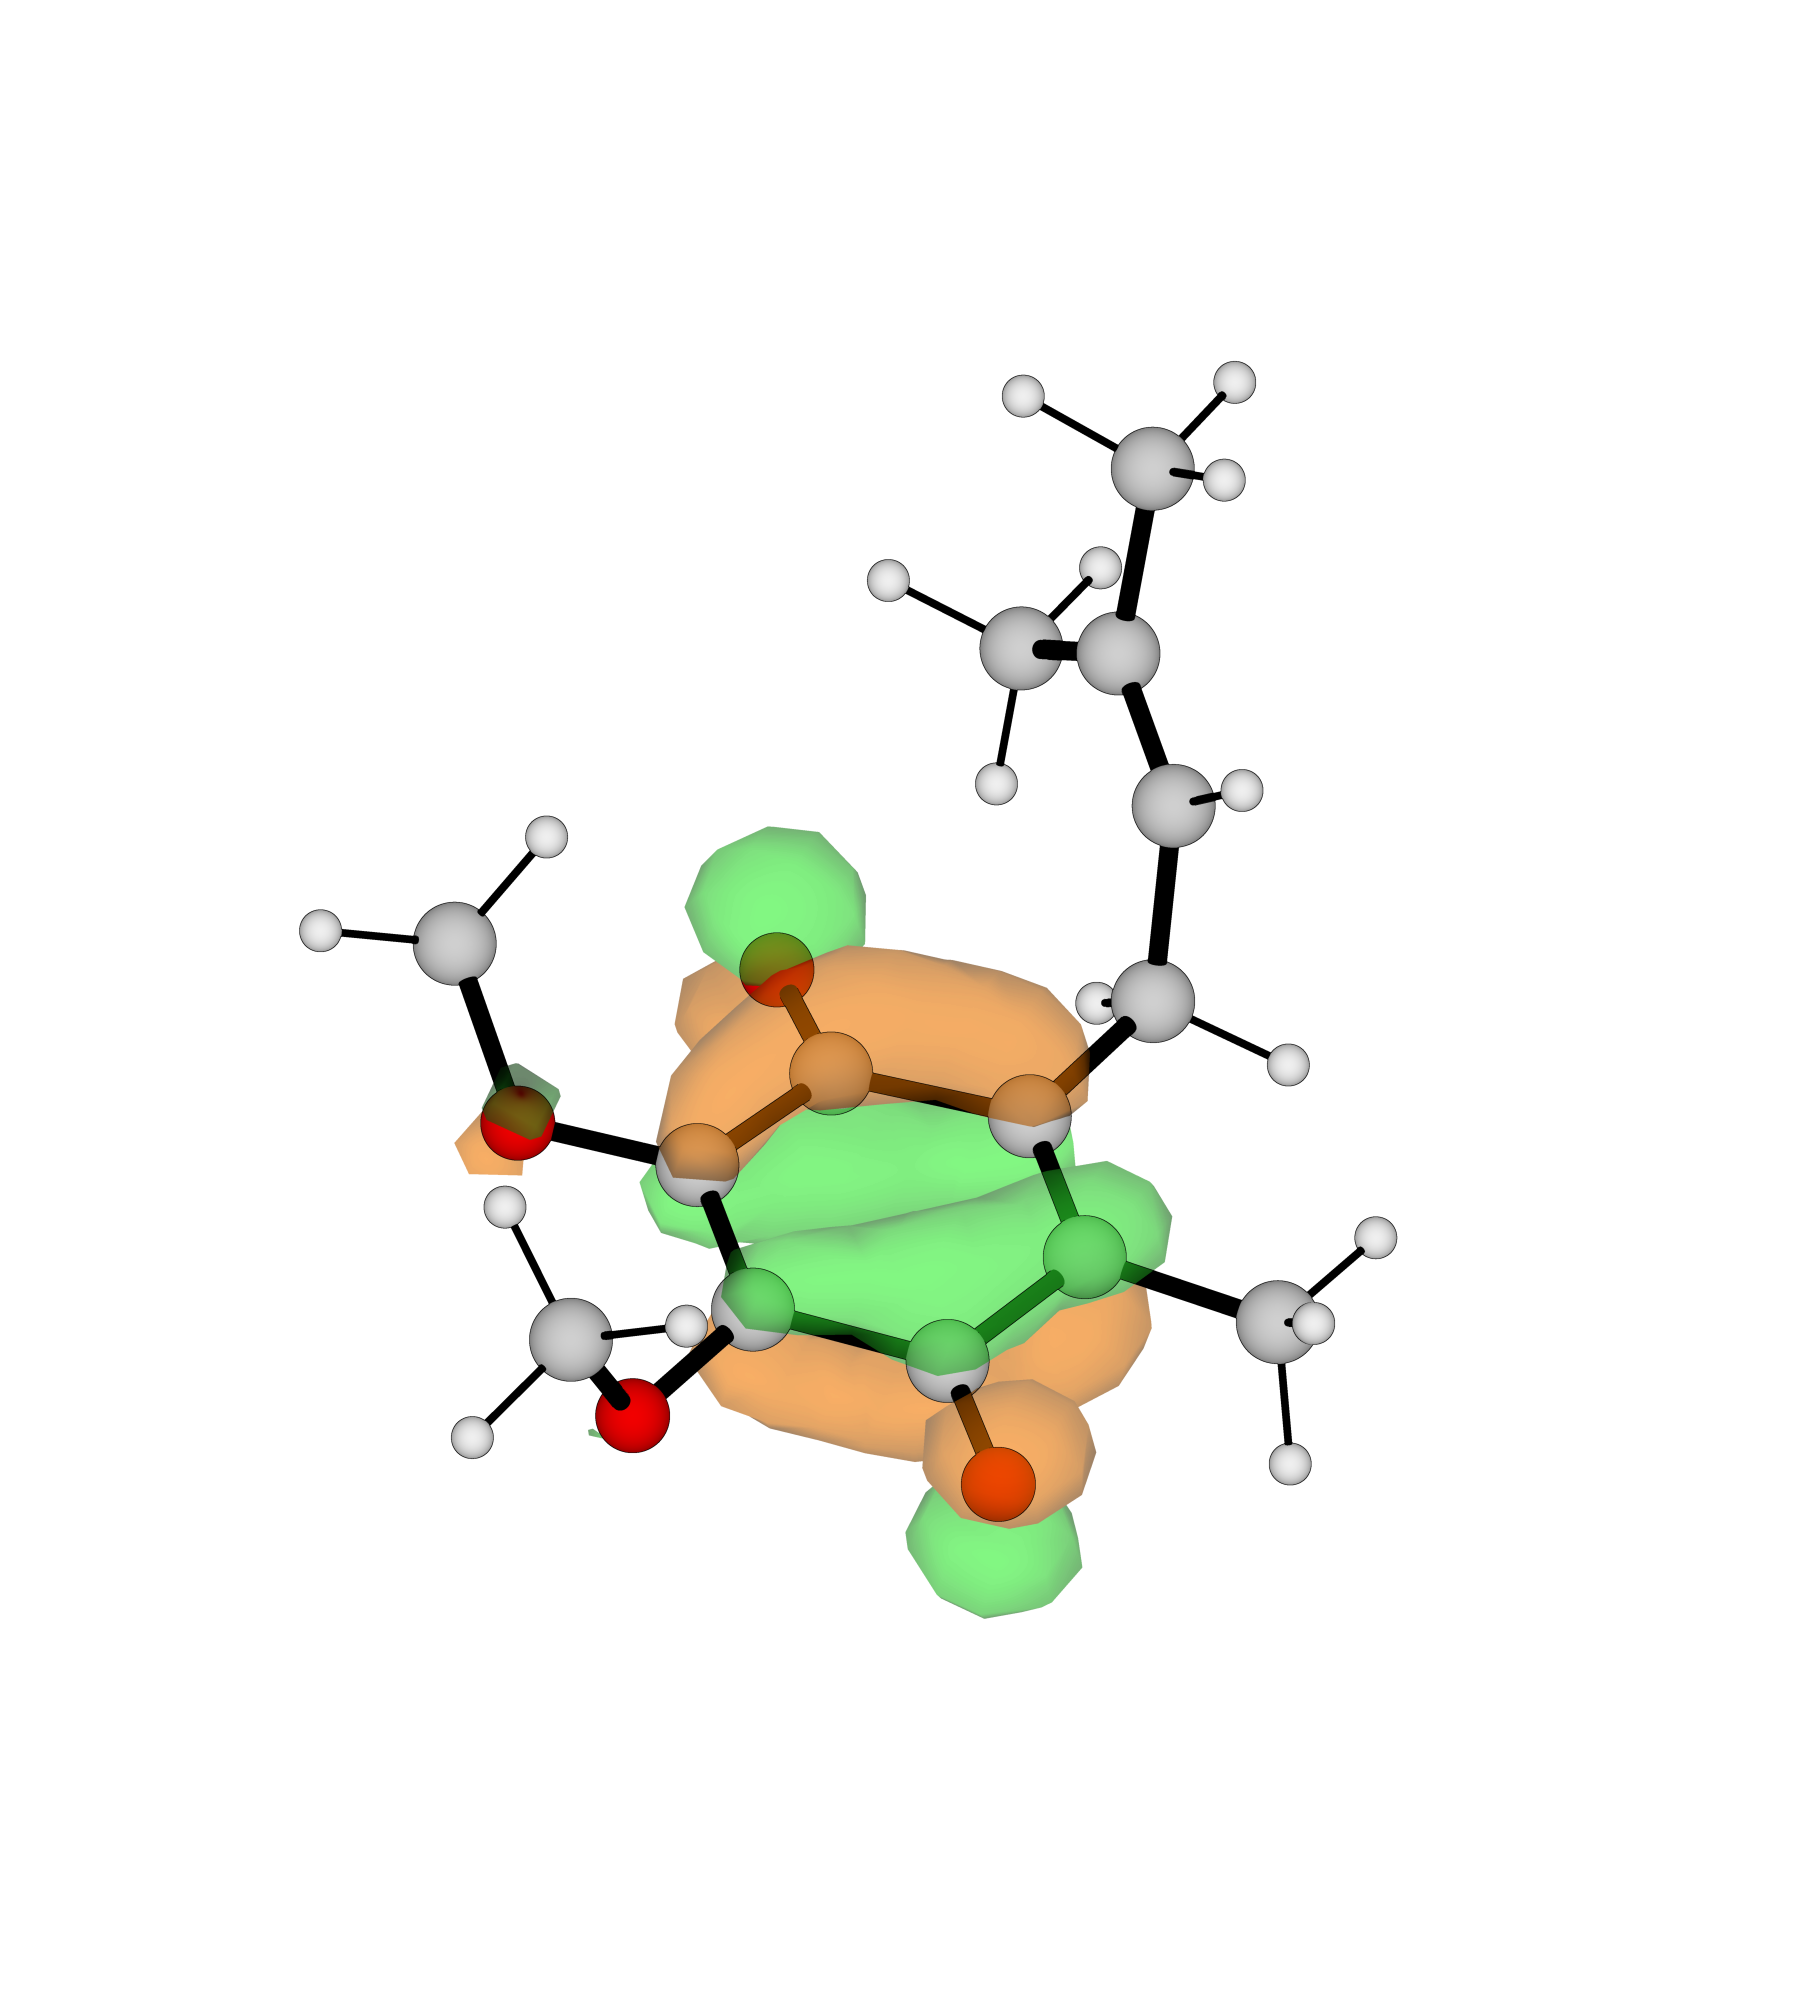
\includegraphics[width=0.6\textwidth]{Figs/cover_VBA.png}}
	%\Put(150,-535){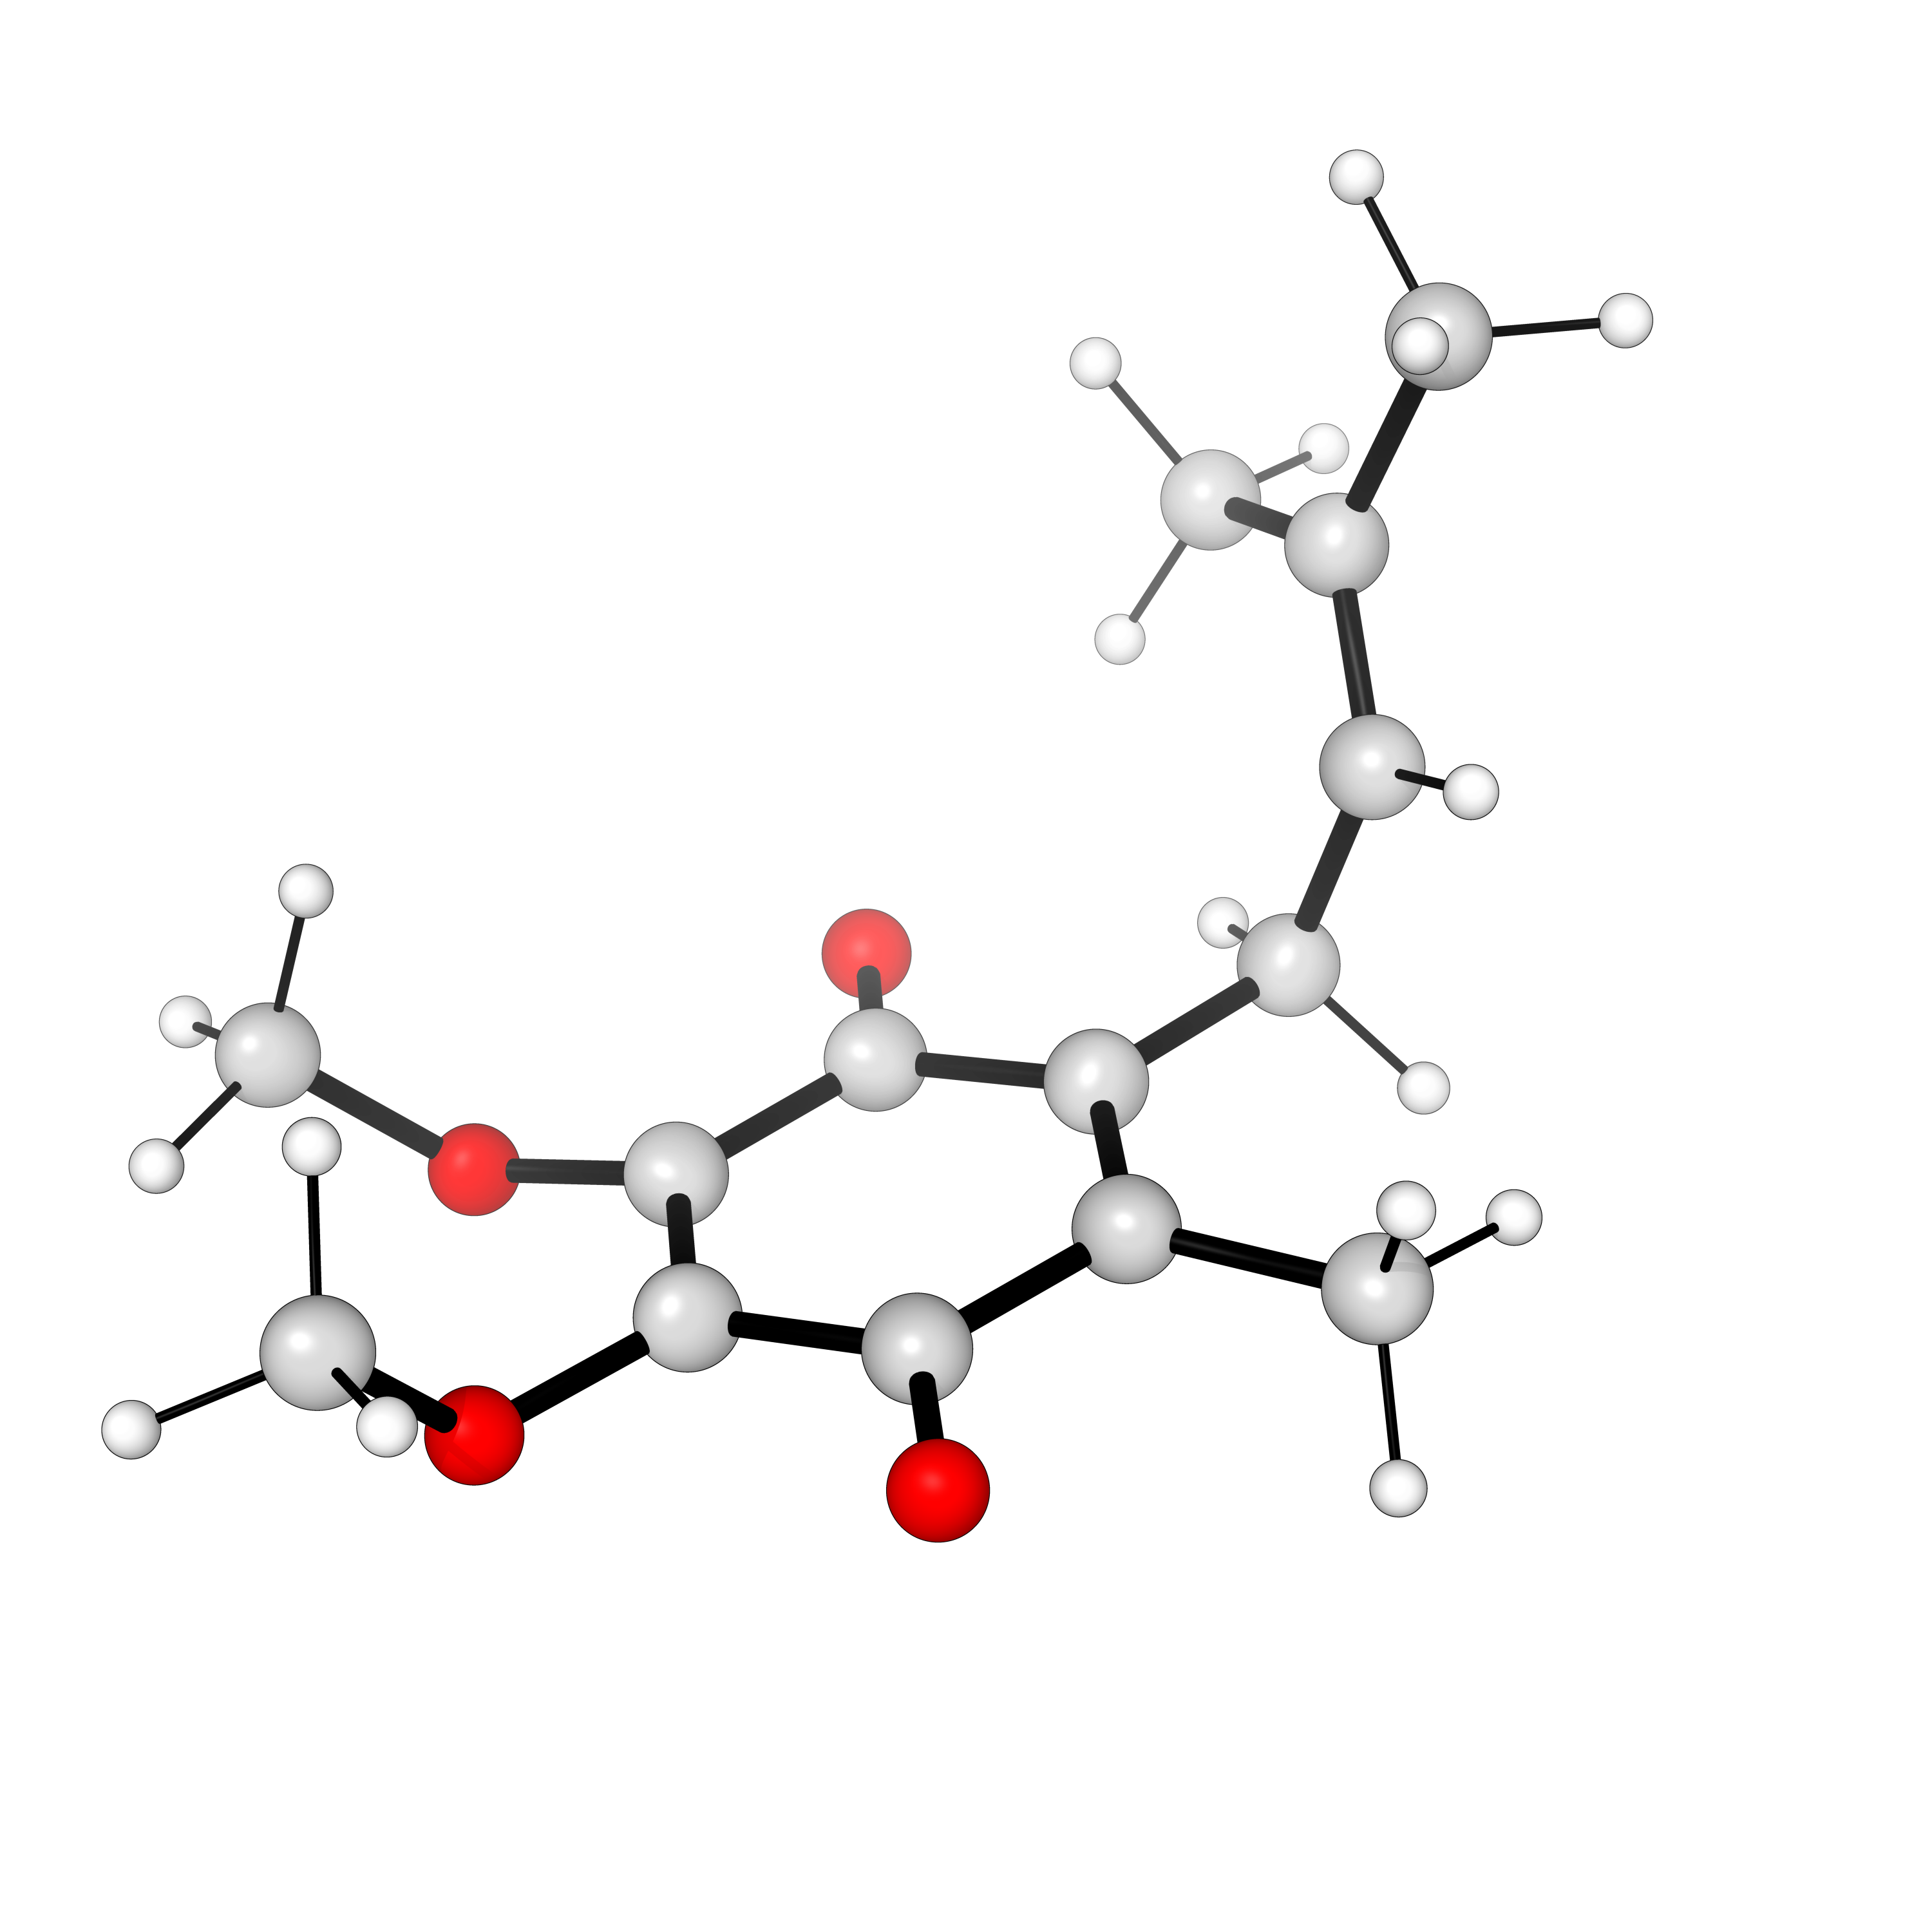
\includegraphics[width=0.6\textwidth]{Figs/uQ.png}}
\end{frame}

% --- New Slide: What is an anion? ---

\begin{frame}{\huge What is an anion?}\large
    \vspace{5pt}
    An anion is a \textbf{negatively charged ion}, formed when an atom or molecule gains one or more electrons. \\
	They are fundamental in chemistry, biology, and materials science and play key roles in almost all chemical processes, including:
        \begin{itemize}
            \item Acid-base chemistry
            \item Redox reactions
            \item Biological processes 
            \item Environmental and atmospheric chemistry
        \end{itemize}
	\begin{flushleft}
	\end{flushleft}
	\vspace{-0.8cm}
    \centering
	\begin{tikzpicture}[scale=1]
		% Neutral molecule
		\node (neutral) at (0,0) {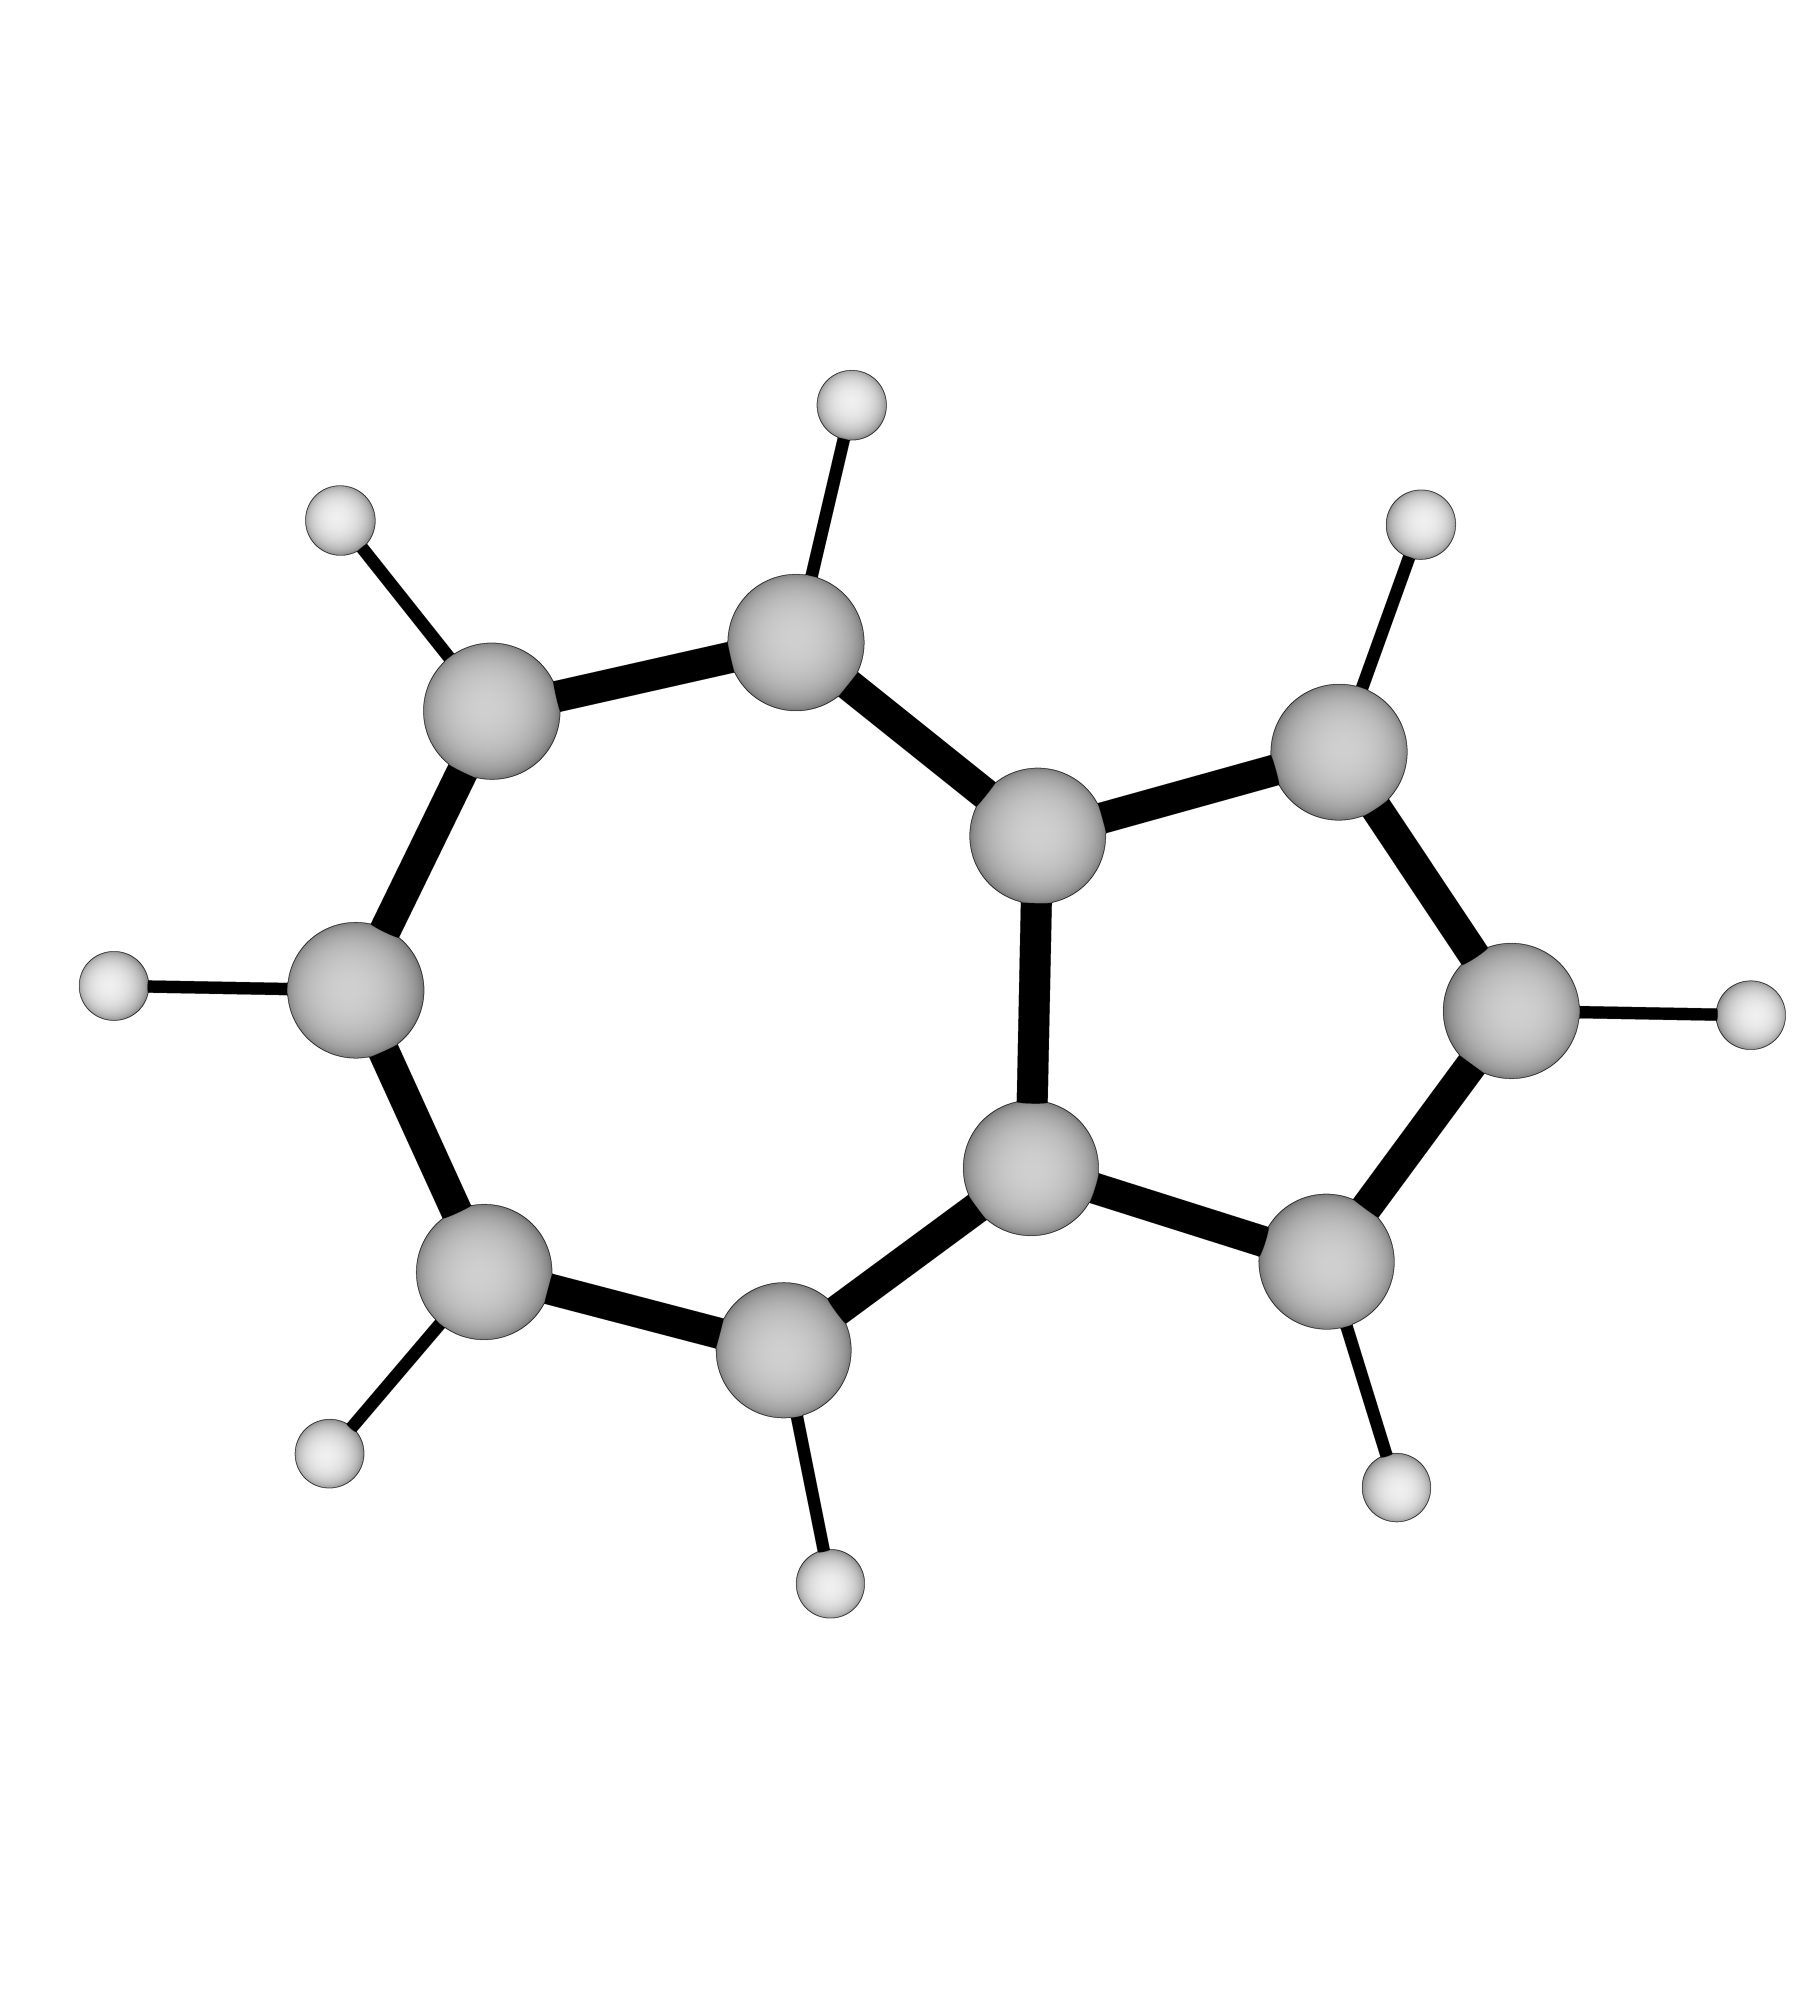
\includegraphics[width=0.25\textwidth]{Figs/azulene_str.png}};
		\node at (0,1.4) {\small Neutral azulene};

		% Electron arrow
		\draw[->, thick, black] (1.8,0) -- (3.2,0) node[midway, above, xshift=0.2cm] {};
		% Electron symbol
		\node[blue] at (2.5,0.4) {\large $+~e^-$};

		% Anion molecule
		\node (anion) at (5,0) {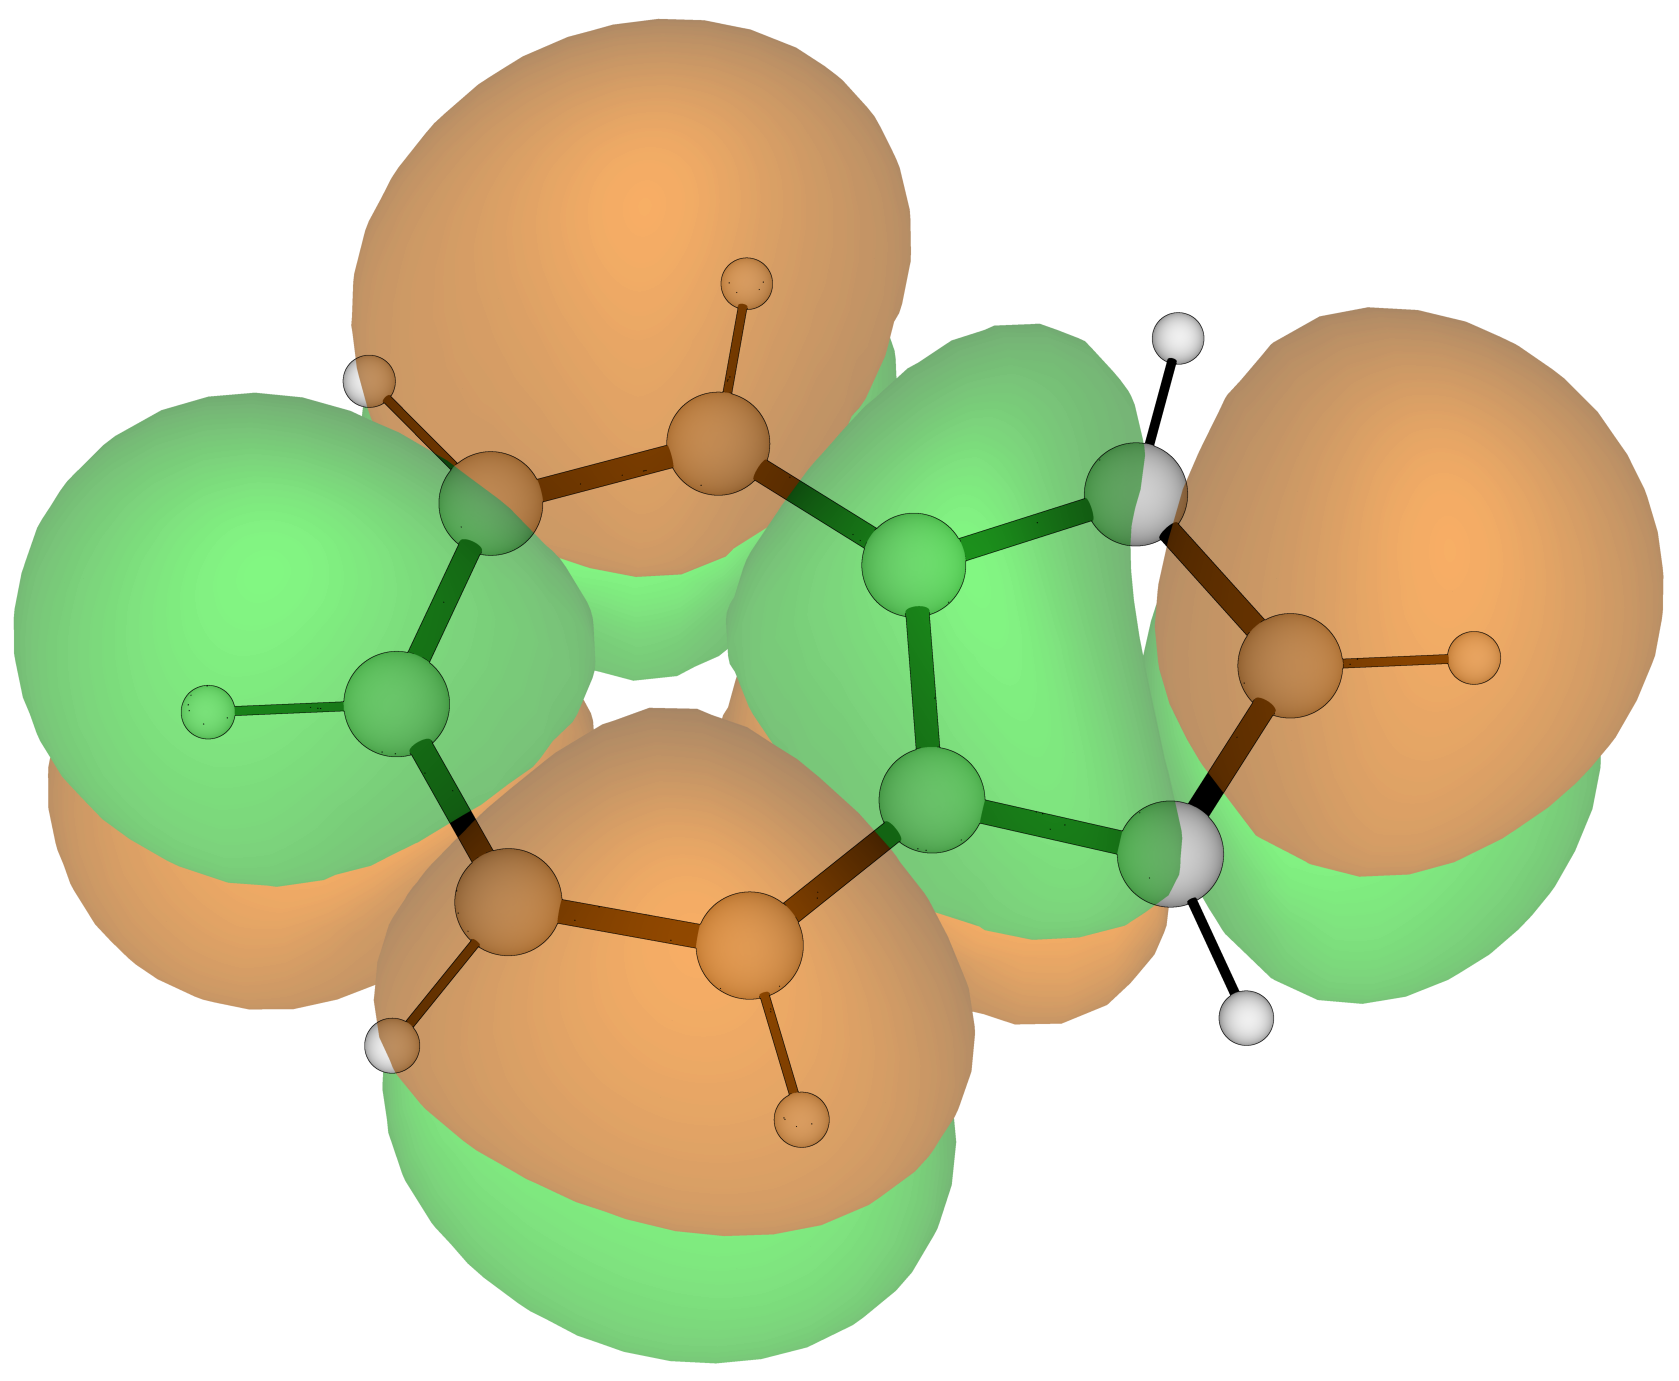
\includegraphics[width=0.25\textwidth]{Figs/azulene.png}};
		\node[blue] at (6,1) {\large $-$};
		\node at (5,1.4) {\small Azulene anion};
	\end{tikzpicture}\\
	\vspace{-0.5cm}
	One can distinguish between valence and non-valence anions.
\end{frame}

% --- Modified Slide: Valence anions ---

\begin{frame}{\huge Valence anions}\large
    \vspace{5pt}
    The extra electron occupies a valence orbital (localised on the molecule).
    These are the most common type of anions (e.g., Cl$^-$, NO$_2^-$).
    \vfill
    \centering
    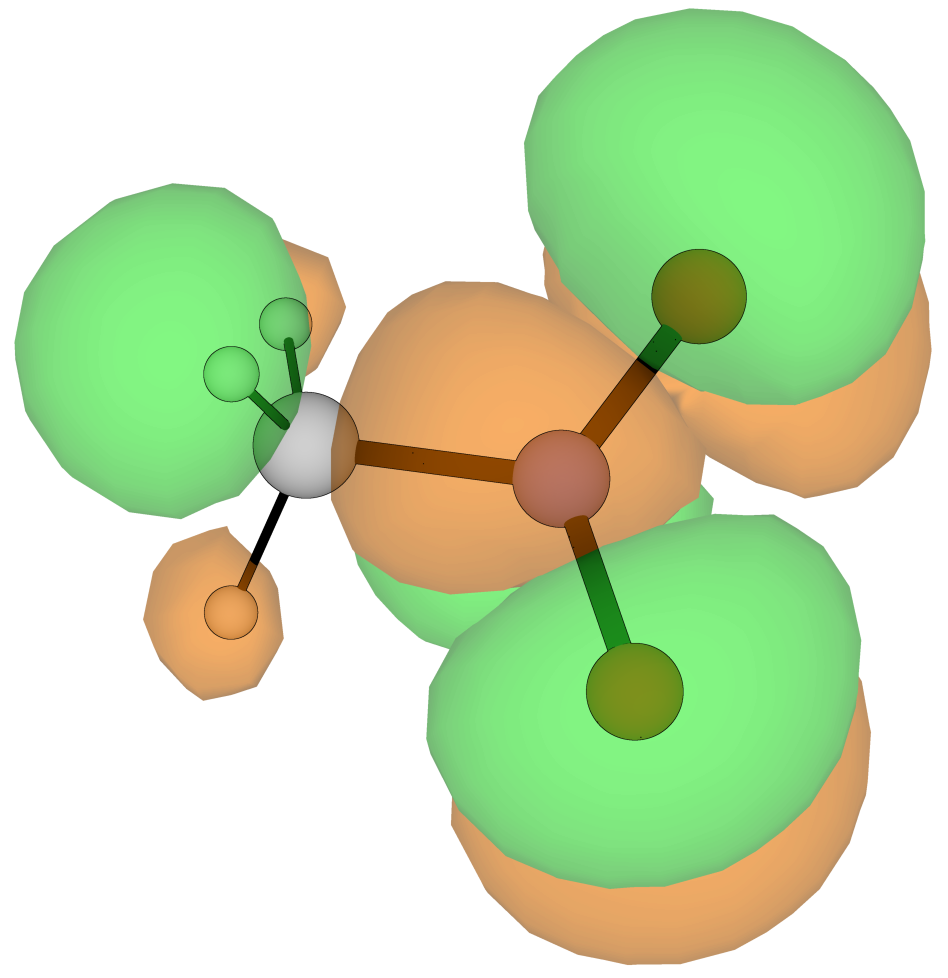
\includegraphics[width=0.3\textwidth]{Figs/MeNO2_VBS.png}\\
	\vspace{10pt}
	\small Valence-bound anion of nitromethane
\end{frame}

\begin{frame}{\huge Non-valence anions}\large
    \vspace{5pt}
	The excess electron is bound by long-range forces (e.g., dipole, quadrupole). The `extra' electron density is located far from the molecule.\\
	Found in atmospheric, interstellar, and biological environments; they act as `doorway' states for electron attachment. 
    \begin{itemize} 

            \item Extremely diffuse electron clouds
            \item Sensitive to correlation and environmental effects
            \item Difficult to describe theoretically
    \end{itemize}
    \vspace{5pt}
	\begin{columns}
		\begin{column}{0.27\textwidth}
			\centering
			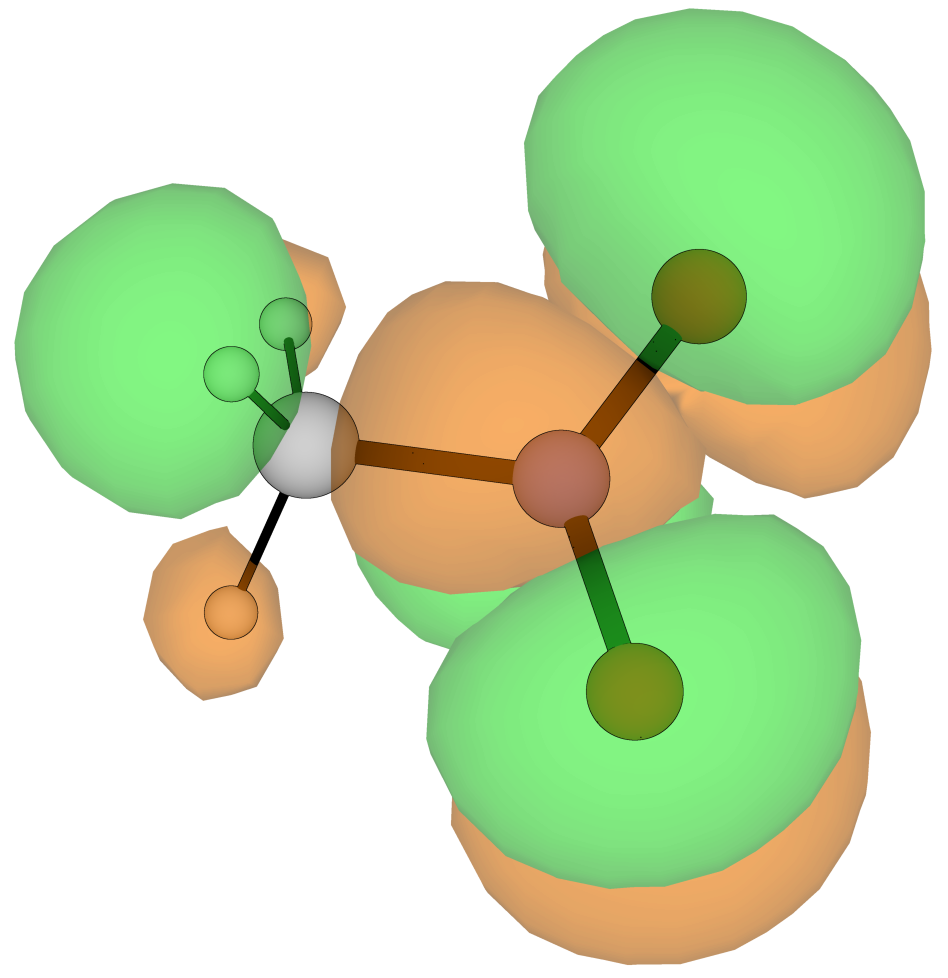
\includegraphics[width=0.7\textwidth]{Figs/MeNO2_VBS.png}\\
			\vspace{3pt}
			\small Valence-bound anion of nitromethane
		\end{column}
		\begin{column}{0.3\textwidth}
			\centering
			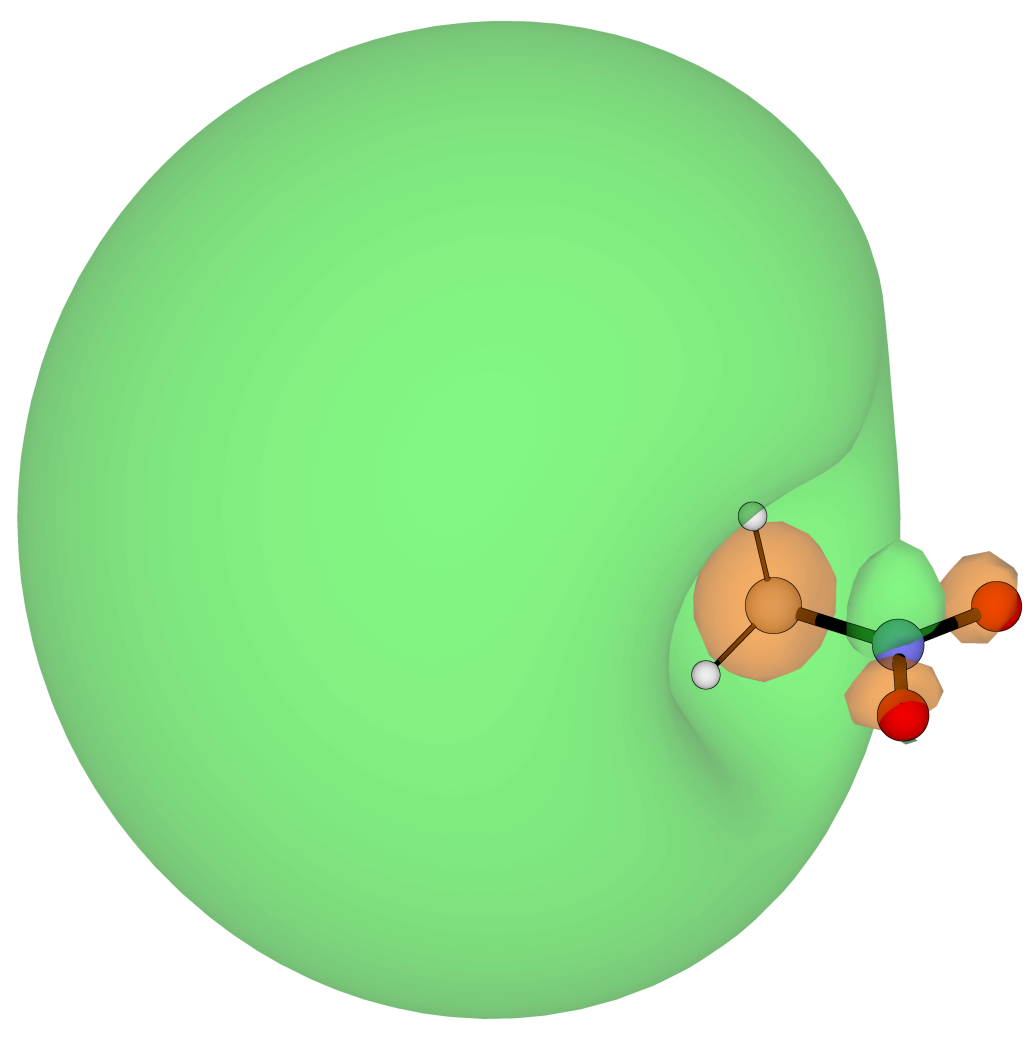
\includegraphics[width=0.7\textwidth]{Figs/MeNO2_DBS.png}\\
			\vspace{3pt}
    		\small Dipole-bound anion of nitromethane
		\end{column}
		\begin{column}{0.27\textwidth}
			\centering
			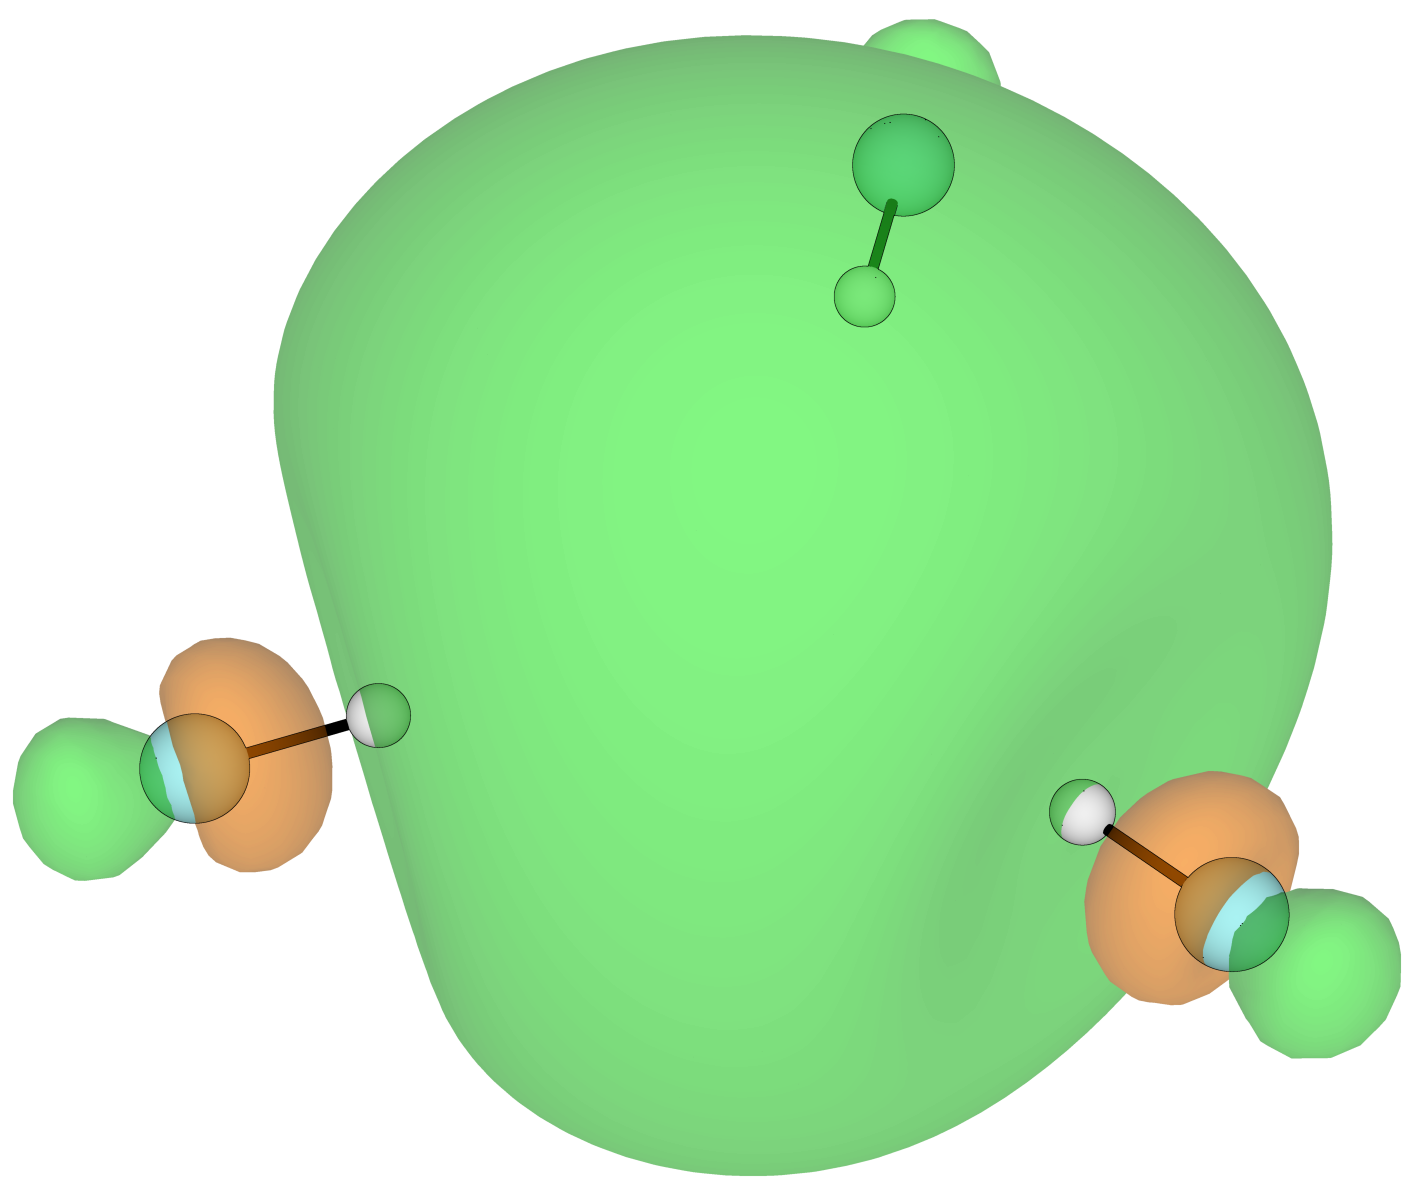
\includegraphics[width=\textwidth]{Figs/hf3.png}\\
			\vspace{3pt}
			\small (HF)\textsubscript{3} solvated electron
		\end{column}	
	\end{columns}
\end{frame}

\begin{frame}{\huge EOM-EA}\large
	Equation-of-motion electron-attachment coupled-cluster (EOM-EA-CC) methods are particularly well suited to study non-valence anions
	\vspace{5pt}
	\begin{itemize}
		\item The description is based on the wave function of the parent neutral molecule
	\end{itemize}
	\centering
	\vspace{5pt} 
			\[ \hat{R}_{\mathrm{EA}} = \sum_{a} r^a a_a^\dagger + \frac{1}{2} \sum_{ab} \sum_{i} r_{i}^{ab} a_a^\dagger a_i a_b^\dagger + \dots \]
	%\vspace{5pt}
	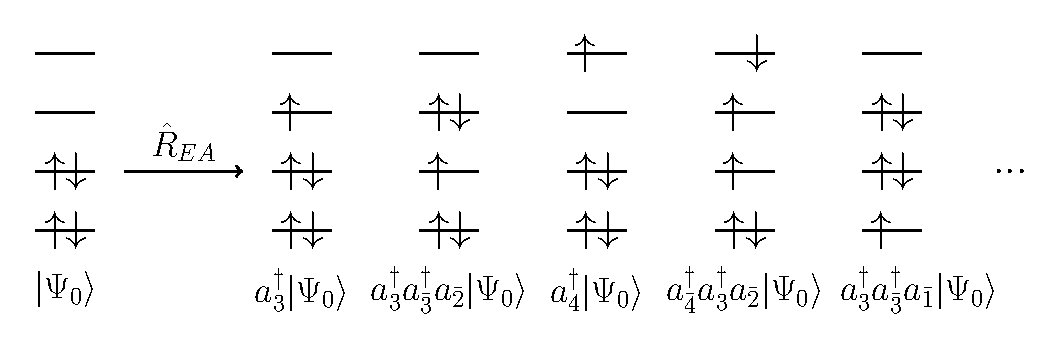
\includegraphics[width=\textwidth]{Figs/EOM_EA.pdf}
\end{frame}

\begin{frame}{\huge Biological Quinones: Ubiquinone (CoQ)}\large
	Quinones are essential electron carriers in biological processes
		\vspace{5pt}
		\begin{itemize}
		%	\item Ubiquinone (coenzyme Q or CoQ) is a component of electron transport chains in bacterial photosynthesis and aerobic respiration.
		\item Component of electron transport chains in bacterial photosynthesis and aerobic respiration	
		\item Capable of both valence and dipole bound anion states
		\end{itemize}
		\begin{columns}[b]
			\begin{column}[b]{0.5\textwidth}
				\centering
				\includegraphics[width=0.8\textwidth]{Figs/Mitochondrial_electron_transport_chain—Etc4.svg.png}\\
				\vspace{3pt}
				\small From Wikimedia Commons
			\end{column}
			\begin{column}[b]{0.25\textwidth}
				\centering
				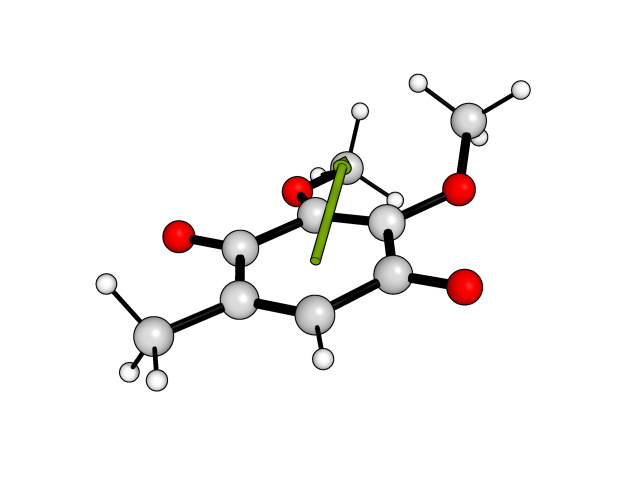
\includegraphics[width=\textwidth]{Figs/Q0_181.png}\\
				\vspace{10pt}
				\small Dipole-bound state
			\end{column}
			\begin{column}[b]{0.25\textwidth}
				\centering
				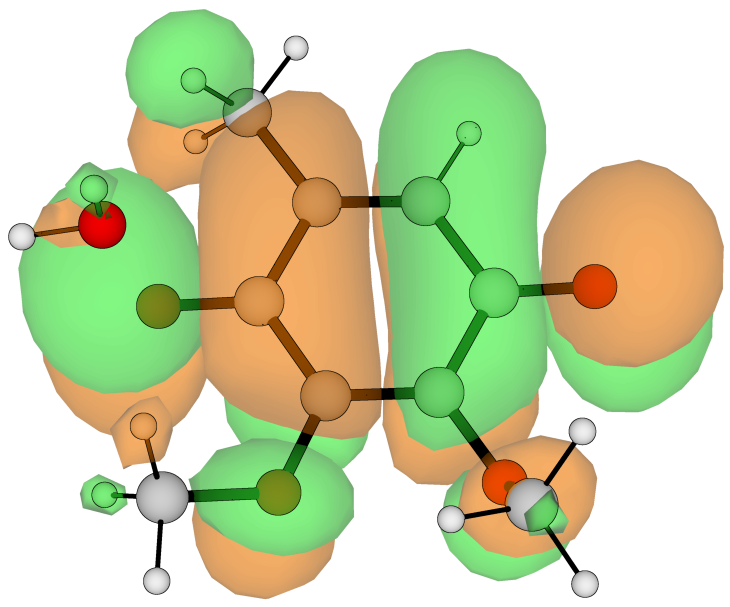
\includegraphics[width=\textwidth]{Figs/Q0_H2O_VBS.png}\\
				\vspace{25pt}
				\small Valence-bound state
			\end{column}
		\end{columns}
\end{frame}

\begin{frame}{\huge Quinone structure}\large
	Each part of the molecule plays a distinct function:
	\begin{itemize}
		\item Quinone head involved in the electron transfer
		\item Isoprenoid tail responsible for the solubility in the membrane
		\item Methoxy chains determine the dipole moment
	\end{itemize}
	\Put(-30,-265){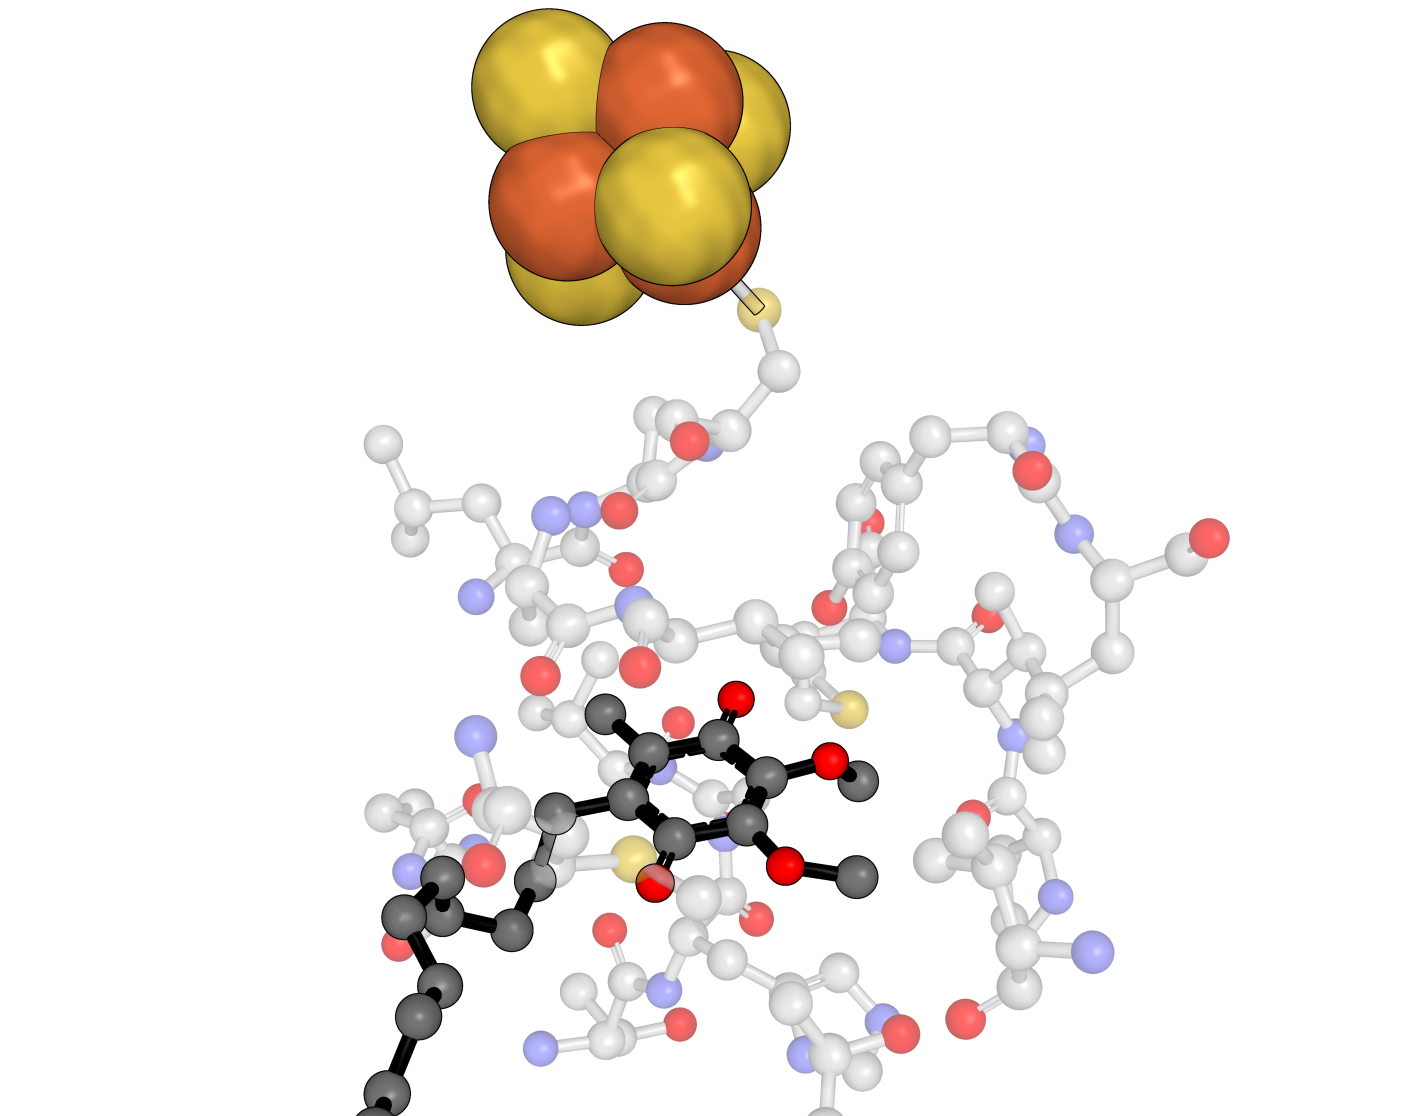
\includegraphics[width=0.55\textwidth]{Figs/uQ_6i0d.png}}
	\Put(85,-285){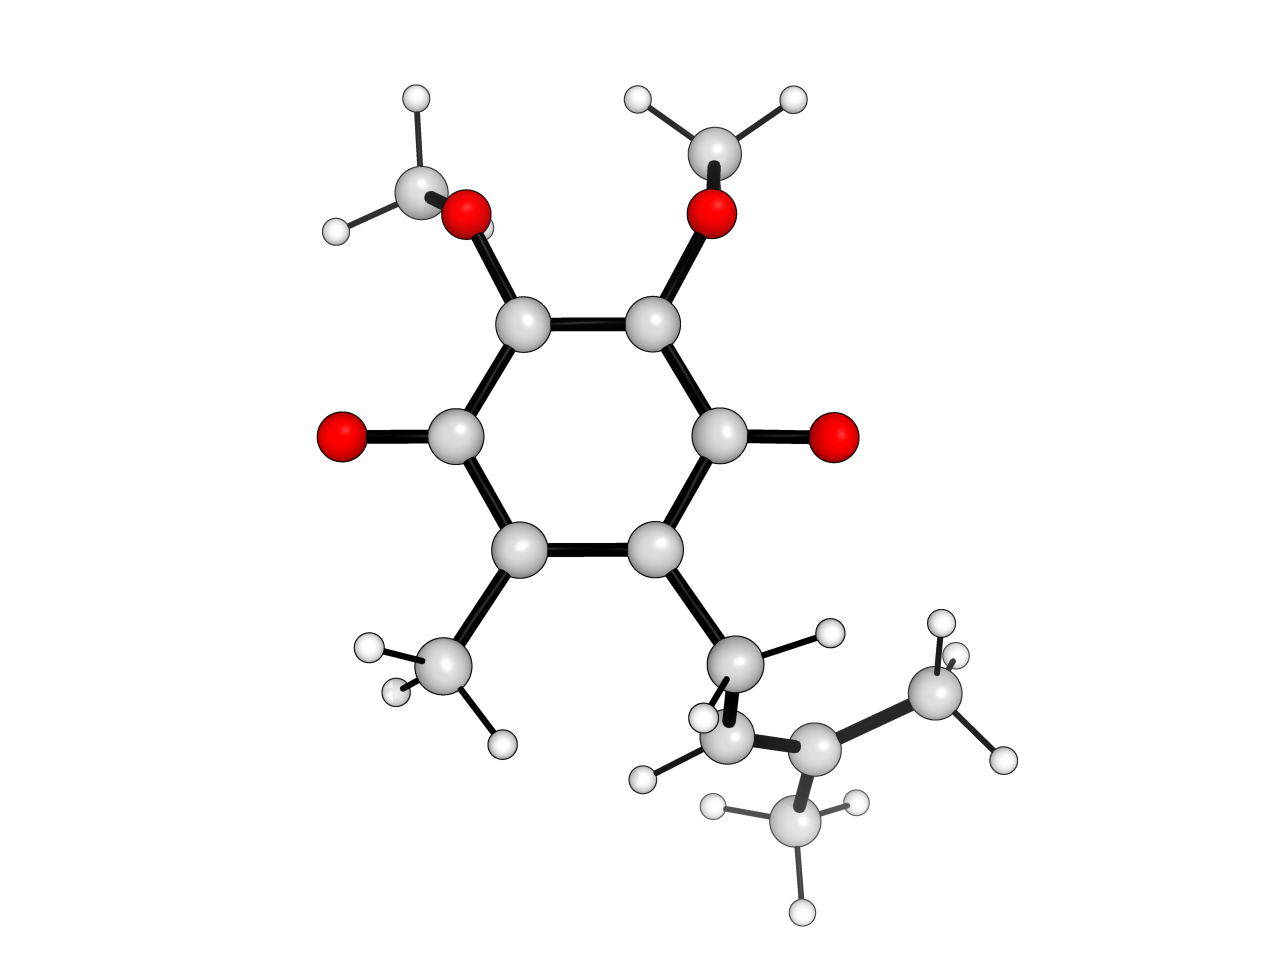
\includegraphics[width=0.57\textwidth]{Figs/Q1.png}}
	\Put(200,-238){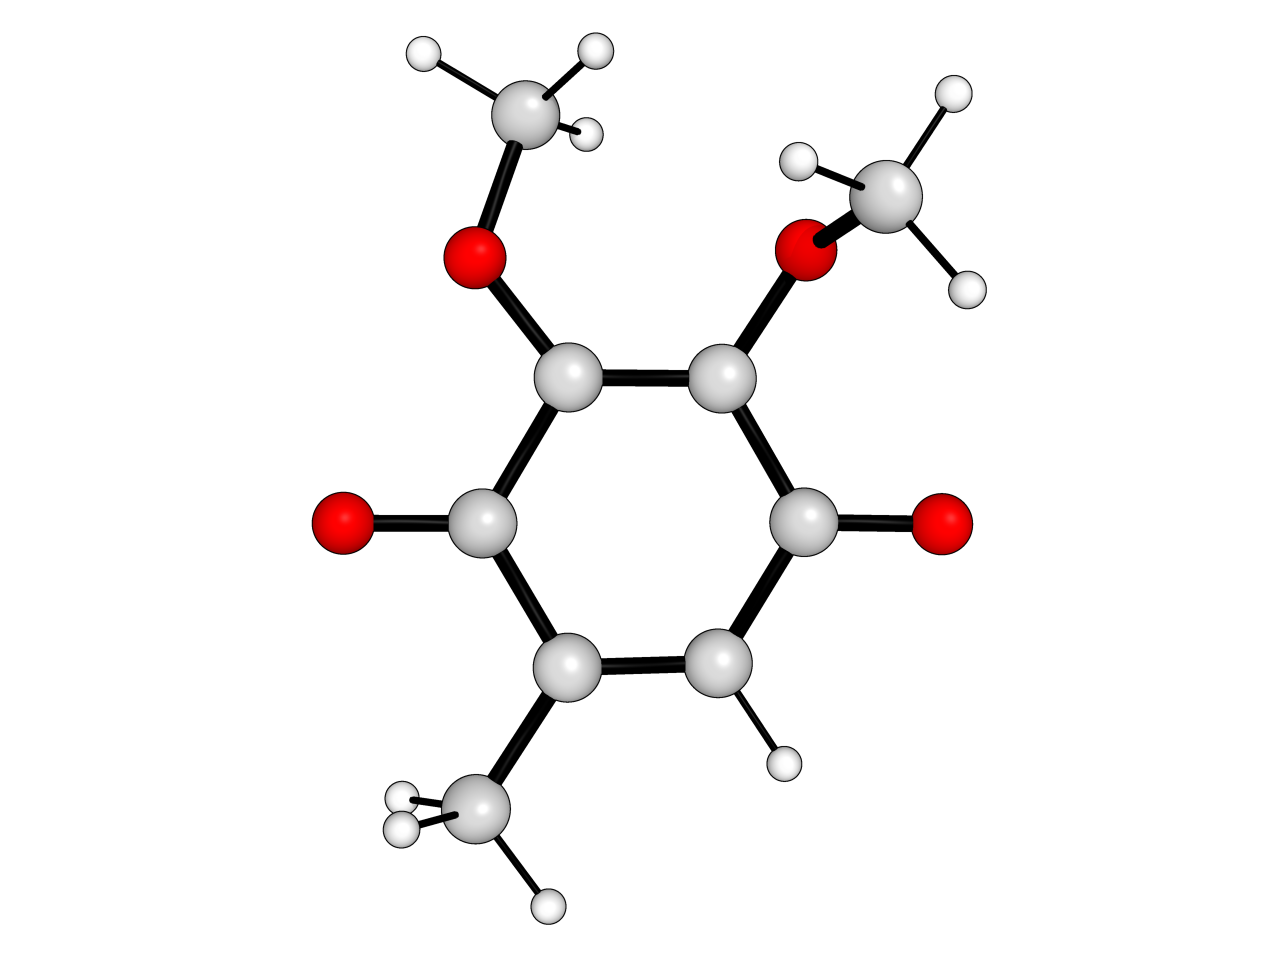
\includegraphics[width=0.465\textwidth]{Figs/Q0189.png}}

	\Put(20,-265){\fontsize{8}{4}\selectfont\text{Q10, Cluster Model}}
	\Put(80,-235){\fontsize{5}{4}\selectfont\text{PDB: 6I0D}}
	\Put(165,-265){\fontsize{8}{4}\selectfont\color{darkgray}\text{Q1}}
	\Put(270,-265){\fontsize{8}{4}\selectfont\color{darkgray}\text{Q0}}
\end{frame}

\begin{frame}{\huge Potential Energy Surface}\large
	We can construct surfaces from the methoxy rotations ($\Psi$ and $\Phi$) of the Q0 model.
	\begin{columns}
		\begin{column}[c]{0.5\textwidth}
			\centering
			% GNUPLOT: LaTeX picture with Postscript
\begingroup
  \makeatletter
  \providecommand\color[2][]{%
    \GenericError{(gnuplot) \space\space\space\@spaces}{%
      Package color not loaded in conjunction with
      terminal option `colourtext'%
    }{See the gnuplot documentation for explanation.%
    }{Either use 'blacktext' in gnuplot or load the package
      color.sty in LaTeX.}%
    \renewcommand\color[2][]{}%
  }%
  \providecommand\includegraphics[2][]{%
    \GenericError{(gnuplot) \space\space\space\@spaces}{%
      Package graphicx or graphics not loaded%
    }{See the gnuplot documentation for explanation.%
    }{The gnuplot epslatex terminal needs graphicx.sty or graphics.sty.}%
    \renewcommand\includegraphics[2][]{}%
  }%
  \providecommand\rotatebox[2]{#2}%
  \@ifundefined{ifGPcolor}{%
    \newif\ifGPcolor
    \GPcolortrue
  }{}%
  \@ifundefined{ifGPblacktext}{%
    \newif\ifGPblacktext
    \GPblacktexttrue
  }{}%
  % define a \g@addto@macro without @ in the name:
  \let\gplgaddtomacro\g@addto@macro
  % define empty templates for all commands taking text:
  \gdef\gplbacktext{}%
  \gdef\gplfronttext{}%
  \makeatother
  \ifGPblacktext
    % no textcolor at all
    \def\colorrgb#1{}%
    \def\colorgray#1{}%
  \else
    % gray or color?
    \ifGPcolor
      \def\colorrgb#1{\color[rgb]{#1}}%
      \def\colorgray#1{\color[gray]{#1}}%
      \expandafter\def\csname LTw\endcsname{\color{white}}%
      \expandafter\def\csname LTb\endcsname{\color{black}}%
      \expandafter\def\csname LTa\endcsname{\color{black}}%
      \expandafter\def\csname LT0\endcsname{\color[rgb]{1,0,0}}%
      \expandafter\def\csname LT1\endcsname{\color[rgb]{0,1,0}}%
      \expandafter\def\csname LT2\endcsname{\color[rgb]{0,0,1}}%
      \expandafter\def\csname LT3\endcsname{\color[rgb]{1,0,1}}%
      \expandafter\def\csname LT4\endcsname{\color[rgb]{0,1,1}}%
      \expandafter\def\csname LT5\endcsname{\color[rgb]{1,1,0}}%
      \expandafter\def\csname LT6\endcsname{\color[rgb]{0,0,0}}%
      \expandafter\def\csname LT7\endcsname{\color[rgb]{1,0.3,0}}%
      \expandafter\def\csname LT8\endcsname{\color[rgb]{0.5,0.5,0.5}}%
    \else
      % gray
      \def\colorrgb#1{\color{black}}%
      \def\colorgray#1{\color[gray]{#1}}%
      \expandafter\def\csname LTw\endcsname{\color{white}}%
      \expandafter\def\csname LTb\endcsname{\color{black}}%
      \expandafter\def\csname LTa\endcsname{\color{black}}%
      \expandafter\def\csname LT0\endcsname{\color{black}}%
      \expandafter\def\csname LT1\endcsname{\color{black}}%
      \expandafter\def\csname LT2\endcsname{\color{black}}%
      \expandafter\def\csname LT3\endcsname{\color{black}}%
      \expandafter\def\csname LT4\endcsname{\color{black}}%
      \expandafter\def\csname LT5\endcsname{\color{black}}%
      \expandafter\def\csname LT6\endcsname{\color{black}}%
      \expandafter\def\csname LT7\endcsname{\color{black}}%
      \expandafter\def\csname LT8\endcsname{\color{black}}%
    \fi
  \fi
    \setlength{\unitlength}{0.0500bp}%
    \ifx\gptboxheight\undefined%
      \newlength{\gptboxheight}%
      \newlength{\gptboxwidth}%
      \newsavebox{\gptboxtext}%
    \fi%
    \setlength{\fboxrule}{0.5pt}%
    \setlength{\fboxsep}{1pt}%
    \definecolor{tbcol}{rgb}{1,1,1}%
\begin{picture}(3680.00,3680.00)%
    \gplgaddtomacro\gplbacktext{%
      \csname LTb\endcsname%%
      \put(714,959){\makebox(0,0)[r]{\strut{}$-150$}}%
      \csname LTb\endcsname%%
      \put(714,1314){\makebox(0,0)[r]{\strut{}$-100$}}%
      \csname LTb\endcsname%%
      \put(714,1668){\makebox(0,0)[r]{\strut{}$-50$}}%
      \csname LTb\endcsname%%
      \put(714,2023){\makebox(0,0)[r]{\strut{}$0$}}%
      \csname LTb\endcsname%%
      \put(714,2378){\makebox(0,0)[r]{\strut{}$50$}}%
      \csname LTb\endcsname%%
      \put(714,2732){\makebox(0,0)[r]{\strut{}$100$}}%
      \csname LTb\endcsname%%
      \put(714,3087){\makebox(0,0)[r]{\strut{}$150$}}%
      \csname LTb\endcsname%%
      \put(812,570){\makebox(0,0){\strut{}$-180$}}%
      \csname LTb\endcsname%%
      \put(1237,570){\makebox(0,0){\strut{}$-120$}}%
      \csname LTb\endcsname%%
      \put(1663,570){\makebox(0,0){\strut{}$-60$}}%
      \csname LTb\endcsname%%
      \put(2089,570){\makebox(0,0){\strut{}$0$}}%
      \csname LTb\endcsname%%
      \put(2514,570){\makebox(0,0){\strut{}$60$}}%
      \csname LTb\endcsname%%
      \put(2940,570){\makebox(0,0){\strut{}$120$}}%
      \csname LTb\endcsname%%
      \put(3366,570){\makebox(0,0){\strut{}$180$}}%
    }%
    \gplgaddtomacro\gplfronttext{%
      \csname LTb\endcsname%%
      \put(357,2023){\rotatebox{-270.00}{\makebox(0,0){\normalsize $\Psi$}}}%
      \csname LTb\endcsname%%
      \put(2089,306){\makebox(0,0){\normalsize $\Phi$}}%
      \csname LTb\endcsname%%
      \put(1770,2270){\rotatebox{-65.00}{\makebox(0,0){\strut{}\textcolor{black}{\footnotesize 500}}}}%
      \csname LTb\endcsname%%
      \put(2378,2036){\rotatebox{127.00}{\makebox(0,0){\strut{}\textcolor{black}{\footnotesize 400}}}}%
      \csname LTb\endcsname%%
      \put(1783,1948){\rotatebox{-45.00}{\makebox(0,0){\strut{}\textcolor{black}{\footnotesize 400}}}}%
      \csname LTb\endcsname%%
      \put(2029,2484){\rotatebox{152.00}{\makebox(0,0){\strut{}\textcolor{black}{\footnotesize 300}}}}%
      \csname LTb\endcsname%%
      \put(1885,1759){\rotatebox{-38.00}{\makebox(0,0){\strut{}\textcolor{black}{\footnotesize 300}}}}%
      \csname LTb\endcsname%%
      \put(2670,1883){\rotatebox{110.00}{\makebox(0,0){\strut{}\textcolor{black}{\footnotesize 200}}}}%
      \csname LTb\endcsname%%
      \put(1477,2794){\rotatebox{-167.00}{\makebox(0,0){\strut{}\textcolor{black}{\footnotesize 200}}}}%
      \csname LTb\endcsname%%
      \put(2014,1527){\rotatebox{-32.00}{\makebox(0,0){\strut{}\textcolor{black}{\footnotesize 200}}}}%
      \csname LTb\endcsname%%
      \put(1196,2849){\rotatebox{33.00}{\makebox(0,0){\strut{}\textcolor{black}{\footnotesize 100}}}}%
      \csname LTb\endcsname%%
      \put(2481,2849){\rotatebox{51.00}{\makebox(0,0){\strut{}\textcolor{black}{\footnotesize 100}}}}%
      \csname LTb\endcsname%%
      \put(2699,2098){\rotatebox{-73.00}{\makebox(0,0){\strut{}\textcolor{black}{\footnotesize 100}}}}%
      \csname LTb\endcsname%%
      \put(1241,2426){\rotatebox{-30.00}{\makebox(0,0){\strut{}\textcolor{black}{\footnotesize 100}}}}%
      \csname LTb\endcsname%%
      \put(1284,1230){\rotatebox{-38.00}{\makebox(0,0){\strut{}\textcolor{black}{\footnotesize 100}}}}%
      \csname LTb\endcsname%%
      \put(2572,1068){\rotatebox{-46.00}{\makebox(0,0){\strut{}\textcolor{black}{\footnotesize 100}}}}%
      \csname LTb\endcsname%%
      \put(962,2336){\rotatebox{-155.00}{\makebox(0,0){\strut{}\textcolor{black}{\footnotesize 50}}}}%
      \csname LTb\endcsname%%
      \put(2958,2287){\rotatebox{-162.00}{\makebox(0,0){\strut{}\textcolor{black}{\footnotesize 50}}}}%
      \csname LTb\endcsname%%
      \put(1820,2873){\rotatebox{-46.00}{\makebox(0,0){\strut{}\textcolor{black}{\footnotesize 50}}}}%
      \csname LTb\endcsname%%
      \put(1885,1197){\rotatebox{49.00}{\makebox(0,0){\strut{}\textcolor{black}{\footnotesize 50}}}}%
    }%
    \gplbacktext
    \put(0,0){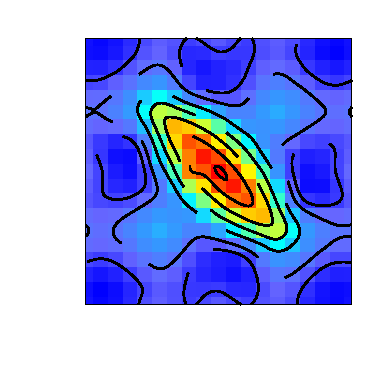
\includegraphics[width={184.00bp},height={184.00bp}]{Figs/Q0_E}}%
    \gplfronttext
  \end{picture}%
\endgroup

			\vspace{10pt}
		\end{column}
		\begin{column}[c]{0.5\textwidth}
			\centering
			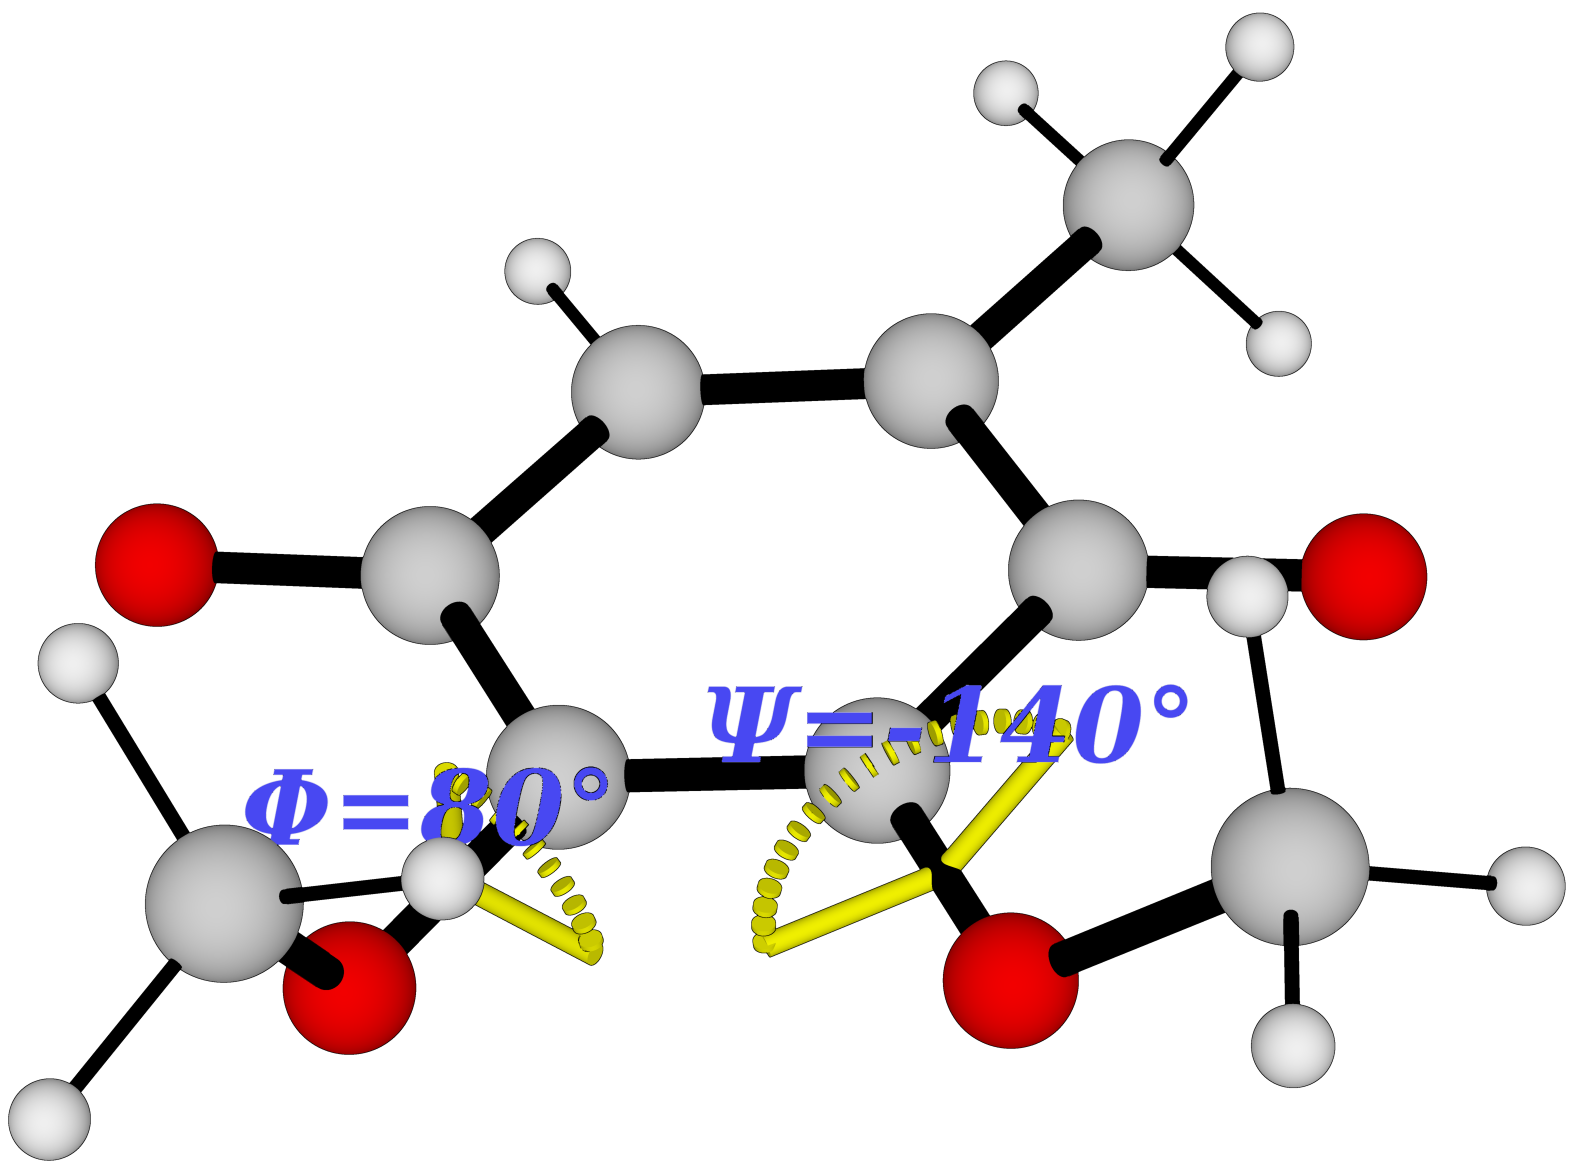
\includegraphics[width=1\textwidth]{Figs/dihedrals.png}
			\vspace{20pt}
		\end{column}
	\end{columns}
\end{frame}

\begin{frame}{\huge Potential Energy Surfaces}\large
	\begin{columns}
		\begin{column}[c]{0.7\textwidth}
			\footnotesize
			% GNUPLOT: LaTeX picture with Postscript
\begingroup
  \makeatletter
  \providecommand\color[2][]{%
    \GenericError{(gnuplot) \space\space\space\@spaces}{%
      Package color not loaded in conjunction with
      terminal option `colourtext'%
    }{See the gnuplot documentation for explanation.%
    }{Either use 'blacktext' in gnuplot or load the package
      color.sty in LaTeX.}%
    \renewcommand\color[2][]{}%
  }%
  \providecommand\includegraphics[2][]{%
    \GenericError{(gnuplot) \space\space\space\@spaces}{%
      Package graphicx or graphics not loaded%
    }{See the gnuplot documentation for explanation.%
    }{The gnuplot epslatex terminal needs graphicx.sty or graphics.sty.}%
    \renewcommand\includegraphics[2][]{}%
  }%
  \providecommand\rotatebox[2]{#2}%
  \@ifundefined{ifGPcolor}{%
    \newif\ifGPcolor
    \GPcolortrue
  }{}%
  \@ifundefined{ifGPblacktext}{%
    \newif\ifGPblacktext
    \GPblacktexttrue
  }{}%
  % define a \g@addto@macro without @ in the name:
  \let\gplgaddtomacro\g@addto@macro
  % define empty templates for all commands taking text:
  \gdef\gplbacktext{}%
  \gdef\gplfronttext{}%
  \makeatother
  \ifGPblacktext
    % no textcolor at all
    \def\colorrgb#1{}%
    \def\colorgray#1{}%
  \else
    % gray or color?
    \ifGPcolor
      \def\colorrgb#1{\color[rgb]{#1}}%
      \def\colorgray#1{\color[gray]{#1}}%
      \expandafter\def\csname LTw\endcsname{\color{white}}%
      \expandafter\def\csname LTb\endcsname{\color{black}}%
      \expandafter\def\csname LTa\endcsname{\color{black}}%
      \expandafter\def\csname LT0\endcsname{\color[rgb]{1,0,0}}%
      \expandafter\def\csname LT1\endcsname{\color[rgb]{0,1,0}}%
      \expandafter\def\csname LT2\endcsname{\color[rgb]{0,0,1}}%
      \expandafter\def\csname LT3\endcsname{\color[rgb]{1,0,1}}%
      \expandafter\def\csname LT4\endcsname{\color[rgb]{0,1,1}}%
      \expandafter\def\csname LT5\endcsname{\color[rgb]{1,1,0}}%
      \expandafter\def\csname LT6\endcsname{\color[rgb]{0,0,0}}%
      \expandafter\def\csname LT7\endcsname{\color[rgb]{1,0.3,0}}%
      \expandafter\def\csname LT8\endcsname{\color[rgb]{0.5,0.5,0.5}}%
    \else
      % gray
      \def\colorrgb#1{\color{black}}%
      \def\colorgray#1{\color[gray]{#1}}%
      \expandafter\def\csname LTw\endcsname{\color{white}}%
      \expandafter\def\csname LTb\endcsname{\color{black}}%
      \expandafter\def\csname LTa\endcsname{\color{black}}%
      \expandafter\def\csname LT0\endcsname{\color{black}}%
      \expandafter\def\csname LT1\endcsname{\color{black}}%
      \expandafter\def\csname LT2\endcsname{\color{black}}%
      \expandafter\def\csname LT3\endcsname{\color{black}}%
      \expandafter\def\csname LT4\endcsname{\color{black}}%
      \expandafter\def\csname LT5\endcsname{\color{black}}%
      \expandafter\def\csname LT6\endcsname{\color{black}}%
      \expandafter\def\csname LT7\endcsname{\color{black}}%
      \expandafter\def\csname LT8\endcsname{\color{black}}%
    \fi
  \fi
    \setlength{\unitlength}{0.0500bp}%
    \ifx\gptboxheight\undefined%
      \newlength{\gptboxheight}%
      \newlength{\gptboxwidth}%
      \newsavebox{\gptboxtext}%
    \fi%
    \setlength{\fboxrule}{0.5pt}%
    \setlength{\fboxsep}{1pt}%
    \definecolor{tbcol}{rgb}{1,1,1}%
\begin{picture}(9060.00,9060.00)%
    \gplgaddtomacro\gplbacktext{%
    }%
    \gplgaddtomacro\gplfronttext{%
      \csname LTb\endcsname%%
      \put(444,5102){\makebox(0,0)[r]{\strut{}$-160$}}%
      \csname LTb\endcsname%%
      \put(444,5544){\makebox(0,0)[r]{\strut{}$-120$}}%
      \csname LTb\endcsname%%
      \put(444,5986){\makebox(0,0)[r]{\strut{}$-80$}}%
      \csname LTb\endcsname%%
      \put(444,6428){\makebox(0,0)[r]{\strut{}$-40$}}%
      \csname LTb\endcsname%%
      \put(444,6870){\makebox(0,0)[r]{\strut{}$0$}}%
      \csname LTb\endcsname%%
      \put(444,7312){\makebox(0,0)[r]{\strut{}$40$}}%
      \csname LTb\endcsname%%
      \put(444,7754){\makebox(0,0)[r]{\strut{}$80$}}%
      \csname LTb\endcsname%%
      \put(444,8196){\makebox(0,0)[r]{\strut{}$120$}}%
      \csname LTb\endcsname%%
      \put(444,8638){\makebox(0,0)[r]{\strut{}$160$}}%
      \csname LTb\endcsname%%
      \put(542,4705){\makebox(0,0){\strut{}}}%
      \csname LTb\endcsname%%
      \put(1205,4705){\makebox(0,0){\strut{}}}%
      \csname LTb\endcsname%%
      \put(1868,4705){\makebox(0,0){\strut{}}}%
      \csname LTb\endcsname%%
      \put(2531,4705){\makebox(0,0){\strut{}}}%
      \csname LTb\endcsname%%
      \put(3194,4705){\makebox(0,0){\strut{}}}%
      \csname LTb\endcsname%%
      \put(3857,4705){\makebox(0,0){\strut{}}}%
      \csname LTb\endcsname%%
      \put(4520,4705){\makebox(0,0){\strut{}}}%
      \csname LTb\endcsname%%
      \put(87,6870){\rotatebox{-270.00}{\makebox(0,0){\normalsize $\Psi$}}}%
      \csname LTb\endcsname%%
      \put(2089,7154){\rotatebox{-66.00}{\makebox(0,0){\strut{}\textcolor{black}{\footnotesize 500}}}}%
      \csname LTb\endcsname%%
      \put(2907,6987){\rotatebox{130.00}{\makebox(0,0){\strut{}\textcolor{black}{\footnotesize 400}}}}%
      \csname LTb\endcsname%%
      \put(2146,6682){\rotatebox{-27.00}{\makebox(0,0){\strut{}\textcolor{black}{\footnotesize 400}}}}%
      \csname LTb\endcsname%%
      \put(2313,7650){\rotatebox{154.00}{\makebox(0,0){\strut{}\textcolor{black}{\footnotesize 300}}}}%
      \csname LTb\endcsname%%
      \put(2302,6385){\rotatebox{-39.00}{\makebox(0,0){\strut{}\textcolor{black}{\footnotesize 300}}}}%
      \csname LTb\endcsname%%
      \put(3383,6779){\rotatebox{113.00}{\makebox(0,0){\strut{}\textcolor{black}{\footnotesize 200}}}}%
      \csname LTb\endcsname%%
      \put(1472,8023){\rotatebox{-143.00}{\makebox(0,0){\strut{}\textcolor{black}{\footnotesize 200}}}}%
      \csname LTb\endcsname%%
      \put(2514,6042){\rotatebox{-26.00}{\makebox(0,0){\strut{}\textcolor{black}{\footnotesize 200}}}}%
      \csname LTb\endcsname%%
      \put(1231,8224){\rotatebox{39.00}{\makebox(0,0){\strut{}\textcolor{black}{\footnotesize 100}}}}%
      \csname LTb\endcsname%%
      \put(3216,8239){\rotatebox{42.00}{\makebox(0,0){\strut{}\textcolor{black}{\footnotesize 100}}}}%
      \csname LTb\endcsname%%
      \put(3517,6877){\rotatebox{-71.00}{\makebox(0,0){\strut{}\textcolor{black}{\footnotesize 100}}}}%
      \csname LTb\endcsname%%
      \put(1307,7421){\rotatebox{-43.00}{\makebox(0,0){\strut{}\textcolor{black}{\footnotesize 100}}}}%
      \csname LTb\endcsname%%
      \put(1378,5563){\rotatebox{-33.00}{\makebox(0,0){\strut{}\textcolor{black}{\footnotesize 100}}}}%
      \csname LTb\endcsname%%
      \put(3383,5294){\rotatebox{-28.00}{\makebox(0,0){\strut{}\textcolor{black}{\footnotesize 100}}}}%
      \csname LTb\endcsname%%
      \put(705,7288){\rotatebox{-112.00}{\makebox(0,0){\strut{}\textcolor{black}{\footnotesize 50}}}}%
      \csname LTb\endcsname%%
      \put(3758,7221){\rotatebox{-149.00}{\makebox(0,0){\strut{}\textcolor{black}{\footnotesize 50}}}}%
      \csname LTb\endcsname%%
      \put(2213,8126){\rotatebox{-28.00}{\makebox(0,0){\strut{}\textcolor{black}{\footnotesize 50}}}}%
      \csname LTb\endcsname%%
      \put(2292,5650){\rotatebox{31.00}{\makebox(0,0){\strut{}\textcolor{black}{\footnotesize 50}}}}%
      \csname LTb\endcsname%%
      \put(2531,8982){\makebox(0,0){\strut{}Conformational Energy (meV)}}%
    }%
    \gplgaddtomacro\gplbacktext{%
    }%
    \gplgaddtomacro\gplfronttext{%
      \csname LTb\endcsname%%
      \put(4874,5102){\makebox(0,0)[r]{\strut{}}}%
      \csname LTb\endcsname%%
      \put(4874,5544){\makebox(0,0)[r]{\strut{}}}%
      \csname LTb\endcsname%%
      \put(4874,5986){\makebox(0,0)[r]{\strut{}}}%
      \csname LTb\endcsname%%
      \put(4874,6428){\makebox(0,0)[r]{\strut{}}}%
      \csname LTb\endcsname%%
      \put(4874,6870){\makebox(0,0)[r]{\strut{}}}%
      \csname LTb\endcsname%%
      \put(4874,7312){\makebox(0,0)[r]{\strut{}}}%
      \csname LTb\endcsname%%
      \put(4874,7754){\makebox(0,0)[r]{\strut{}}}%
      \csname LTb\endcsname%%
      \put(4874,8196){\makebox(0,0)[r]{\strut{}}}%
      \csname LTb\endcsname%%
      \put(4874,8638){\makebox(0,0)[r]{\strut{}}}%
      \csname LTb\endcsname%%
      \put(4971,4705){\makebox(0,0){\strut{}}}%
      \csname LTb\endcsname%%
      \put(5634,4705){\makebox(0,0){\strut{}}}%
      \csname LTb\endcsname%%
      \put(6297,4705){\makebox(0,0){\strut{}}}%
      \csname LTb\endcsname%%
      \put(6960,4705){\makebox(0,0){\strut{}}}%
      \csname LTb\endcsname%%
      \put(7623,4705){\makebox(0,0){\strut{}}}%
      \csname LTb\endcsname%%
      \put(8286,4705){\makebox(0,0){\strut{}}}%
      \csname LTb\endcsname%%
      \put(8949,4705){\makebox(0,0){\strut{}}}%
      \csname LTb\endcsname%%
      \put(5031,7851){\rotatebox{37.00}{\makebox(0,0){\strut{}\textcolor{black}{\footnotesize 3.0}}}}%
      \csname LTb\endcsname%%
      \put(8832,6500){\rotatebox{156.00}{\makebox(0,0){\strut{}\textcolor{black}{\footnotesize 3.0}}}}%
      \csname LTb\endcsname%%
      \put(6547,7260){\rotatebox{-78.00}{\makebox(0,0){\strut{}\textcolor{black}{\footnotesize 2.5}}}}%
      \csname LTb\endcsname%%
      \put(5651,8271){\rotatebox{-7.00}{\makebox(0,0){\strut{}\textcolor{black}{\footnotesize 2.5}}}}%
      \csname LTb\endcsname%%
      \put(5409,6940){\rotatebox{-127.00}{\makebox(0,0){\strut{}\textcolor{black}{\footnotesize 2.5}}}}%
      \csname LTb\endcsname%%
      \put(8618,7519){\rotatebox{-88.00}{\makebox(0,0){\strut{}\textcolor{black}{\footnotesize 2.5}}}}%
      \csname LTb\endcsname%%
      \put(8083,6140){\rotatebox{-101.00}{\makebox(0,0){\strut{}\textcolor{black}{\footnotesize 2.5}}}}%
      \csname LTb\endcsname%%
      \put(5500,6320){\rotatebox{91.00}{\makebox(0,0){\strut{}\textcolor{black}{\footnotesize 2.0}}}}%
      \csname LTb\endcsname%%
      \put(6314,7040){\rotatebox{-47.00}{\makebox(0,0){\strut{}\textcolor{black}{\footnotesize 2.0}}}}%
      \csname LTb\endcsname%%
      \put(7233,6000){\rotatebox{-38.00}{\makebox(0,0){\strut{}\textcolor{black}{\footnotesize 2.0}}}}%
      \csname LTb\endcsname%%
      \put(6531,7999){\rotatebox{-101.00}{\makebox(0,0){\strut{}\textcolor{black}{\footnotesize 2.0}}}}%
      \csname LTb\endcsname%%
      \put(7425,6960){\rotatebox{-59.00}{\makebox(0,0){\strut{}\textcolor{black}{\footnotesize 2.0}}}}%
      \csname LTb\endcsname%%
      \put(8359,7080){\rotatebox{64.00}{\makebox(0,0){\strut{}\textcolor{black}{\footnotesize 2.0}}}}%
      \csname LTb\endcsname%%
      \put(5471,5690){\rotatebox{52.00}{\makebox(0,0){\strut{}\textcolor{black}{\footnotesize 1.5}}}}%
      \csname LTb\endcsname%%
      \put(6291,6706){\rotatebox{-17.00}{\makebox(0,0){\strut{}\textcolor{black}{\footnotesize 1.5}}}}%
      \csname LTb\endcsname%%
      \put(6870,5426){\rotatebox{-106.00}{\makebox(0,0){\strut{}\textcolor{black}{\footnotesize 1.5}}}}%
      \csname LTb\endcsname%%
      \put(7650,8582){\rotatebox{-176.00}{\makebox(0,0){\strut{}\textcolor{black}{\footnotesize 1.5}}}}%
      \csname LTb\endcsname%%
      \put(7238,7519){\rotatebox{-45.00}{\makebox(0,0){\strut{}\textcolor{black}{\footnotesize 1.5}}}}%
      \csname LTb\endcsname%%
      \put(8205,7420){\rotatebox{78.00}{\makebox(0,0){\strut{}\textcolor{black}{\footnotesize 1.5}}}}%
      \csname LTb\endcsname%%
      \put(5771,5854){\rotatebox{56.00}{\makebox(0,0){\strut{}\textcolor{black}{\footnotesize 1.0}}}}%
      \csname LTb\endcsname%%
      \put(6570,5482){\rotatebox{-124.00}{\makebox(0,0){\strut{}\textcolor{black}{\footnotesize 1.0}}}}%
      \csname LTb\endcsname%%
      \put(7490,8350){\rotatebox{-162.00}{\makebox(0,0){\strut{}\textcolor{black}{\footnotesize 1.0}}}}%
      \csname LTb\endcsname%%
      \put(8062,7739){\rotatebox{60.00}{\makebox(0,0){\strut{}\textcolor{black}{\footnotesize 1.0}}}}%
      \csname LTb\endcsname%%
      \put(5883,5721){\rotatebox{-132.00}{\makebox(0,0){\strut{}\textcolor{black}{\footnotesize 0.5}}}}%
      \csname LTb\endcsname%%
      \put(7669,8179){\rotatebox{-140.00}{\makebox(0,0){\strut{}\textcolor{black}{\footnotesize 0.5}}}}%
      \csname LTb\endcsname%%
      \put(6960,8982){\makebox(0,0){Dipole Strength (Debye)}}%
    }%
    \gplgaddtomacro\gplbacktext{%
    }%
    \gplgaddtomacro\gplfronttext{%
      \csname LTb\endcsname%%
      \put(444,763){\makebox(0,0)[r]{\strut{}$-160$}}%
      \csname LTb\endcsname%%
      \put(444,1205){\makebox(0,0)[r]{\strut{}$-120$}}%
      \csname LTb\endcsname%%
      \put(444,1647){\makebox(0,0)[r]{\strut{}$-80$}}%
      \csname LTb\endcsname%%
      \put(444,2089){\makebox(0,0)[r]{\strut{}$-40$}}%
      \csname LTb\endcsname%%
      \put(444,2531){\makebox(0,0)[r]{\strut{}$0$}}%
      \csname LTb\endcsname%%
      \put(444,2973){\makebox(0,0)[r]{\strut{}$40$}}%
      \csname LTb\endcsname%%
      \put(444,3415){\makebox(0,0)[r]{\strut{}$80$}}%
      \csname LTb\endcsname%%
      \put(444,3857){\makebox(0,0)[r]{\strut{}$120$}}%
      \csname LTb\endcsname%%
      \put(444,4298){\makebox(0,0)[r]{\strut{}$160$}}%
      \csname LTb\endcsname%%
      \put(542,366){\makebox(0,0){\strut{}$-180$}}%
      \csname LTb\endcsname%%
      \put(1205,366){\makebox(0,0){\strut{}$-120$}}%
      \csname LTb\endcsname%%
      \put(1868,366){\makebox(0,0){\strut{}$-60$}}%
      \csname LTb\endcsname%%
      \put(2531,366){\makebox(0,0){\strut{}$0$}}%
      \csname LTb\endcsname%%
      \put(3194,366){\makebox(0,0){\strut{}$60$}}%
      \csname LTb\endcsname%%
      \put(3857,366){\makebox(0,0){\strut{}$120$}}%
      \csname LTb\endcsname%%
      \put(4519,366){\makebox(0,0){\strut{}$180$}}%
      \csname LTb\endcsname%%
      \put(87,2531){\rotatebox{-270.00}{\makebox(0,0){\normalsize $\Psi$}}}%
      \csname LTb\endcsname%%
      \put(2531,102){\makebox(0,0){\normalsize $\Phi$}}%
      \csname LTb\endcsname%%
      \put(2390,2781){\rotatebox{150.00}{\makebox(0,0){\strut{}\textcolor{black}{\footnotesize 1.3}}}}%
      \csname LTb\endcsname%%
      \put(2270,2355){\rotatebox{-57.00}{\makebox(0,0){\strut{}\textcolor{black}{\footnotesize 1.4}}}}%
      \csname LTb\endcsname%%
      \put(2912,2859){\rotatebox{124.00}{\makebox(0,0){\strut{}\textcolor{black}{\footnotesize 1.5}}}}%
      \csname LTb\endcsname%%
      \put(2511,1819){\rotatebox{-36.00}{\makebox(0,0){\strut{}\textcolor{black}{\footnotesize 1.5}}}}%
      \csname LTb\endcsname%%
      \put(2052,3555){\rotatebox{51.00}{\makebox(0,0){\strut{}\textcolor{black}{\footnotesize 1.6}}}}%
      \csname LTb\endcsname%%
      \put(2164,1627){\rotatebox{-79.00}{\makebox(0,0){\strut{}\textcolor{black}{\footnotesize 1.6}}}}%
      \csname LTb\endcsname%%
      \put(3435,2928){\rotatebox{-15.00}{\makebox(0,0){\strut{}\textcolor{black}{\footnotesize 1.6}}}}%
      \csname LTb\endcsname%%
      \put(3530,2028){\rotatebox{40.00}{\makebox(0,0){\strut{}\textcolor{black}{\footnotesize 1.6}}}}%
      \csname LTb\endcsname%%
      \put(1814,1426){\rotatebox{-81.00}{\makebox(0,0){\strut{}\textcolor{black}{\footnotesize 1.7}}}}%
      \csname LTb\endcsname%%
      \put(1753,3676){\rotatebox{49.00}{\makebox(0,0){\strut{}\textcolor{black}{\footnotesize 1.7}}}}%
      \csname LTb\endcsname%%
      \put(3475,3295){\rotatebox{-26.00}{\makebox(0,0){\strut{}\textcolor{black}{\footnotesize 1.7}}}}%
      \csname LTb\endcsname%%
      \put(3592,1667){\rotatebox{55.00}{\makebox(0,0){\strut{}\textcolor{black}{\footnotesize 1.7}}}}%
      \csname LTb\endcsname%%
      \put(2531,4643){\makebox(0,0){VBA EA (eV)}}%
    }%
    \gplgaddtomacro\gplbacktext{%
    }%
    \gplgaddtomacro\gplfronttext{%
      \csname LTb\endcsname%%
      \put(4874,763){\makebox(0,0)[r]{\strut{}}}%
      \csname LTb\endcsname%%
      \put(4874,1205){\makebox(0,0)[r]{\strut{}}}%
      \csname LTb\endcsname%%
      \put(4874,1647){\makebox(0,0)[r]{\strut{}}}%
      \csname LTb\endcsname%%
      \put(4874,2089){\makebox(0,0)[r]{\strut{}}}%
      \csname LTb\endcsname%%
      \put(4874,2531){\makebox(0,0)[r]{\strut{}}}%
      \csname LTb\endcsname%%
      \put(4874,2973){\makebox(0,0)[r]{\strut{}}}%
      \csname LTb\endcsname%%
      \put(4874,3415){\makebox(0,0)[r]{\strut{}}}%
      \csname LTb\endcsname%%
      \put(4874,3857){\makebox(0,0)[r]{\strut{}}}%
      \csname LTb\endcsname%%
      \put(4874,4298){\makebox(0,0)[r]{\strut{}}}%
      \csname LTb\endcsname%%
      \put(4971,366){\makebox(0,0){\strut{}$-180$}}%
      \csname LTb\endcsname%%
      \put(5634,366){\makebox(0,0){\strut{}$-120$}}%
      \csname LTb\endcsname%%
      \put(6297,366){\makebox(0,0){\strut{}$-60$}}%
      \csname LTb\endcsname%%
      \put(6960,366){\makebox(0,0){\strut{}$0$}}%
      \csname LTb\endcsname%%
      \put(7623,366){\makebox(0,0){\strut{}$60$}}%
      \csname LTb\endcsname%%
      \put(8286,366){\makebox(0,0){\strut{}$120$}}%
      \csname LTb\endcsname%%
      \put(8949,366){\makebox(0,0){\strut{}$180$}}%
      \csname LTb\endcsname%%
      \put(6960,102){\makebox(0,0){\normalsize $\Phi$}}%
      \csname LTb\endcsname%%
      \put(7021,2310){\rotatebox{-43.00}{\makebox(0,0){\strut{}\textcolor{black}{\footnotesize 12}}}}%
      \csname LTb\endcsname%%
      \put(7236,2069){\rotatebox{-30.00}{\makebox(0,0){\strut{}\textcolor{black}{\footnotesize 9}}}}%
      \csname LTb\endcsname%%
      \put(5255,3234){\rotatebox{-53.00}{\makebox(0,0){\strut{}\textcolor{black}{\footnotesize 6}}}}%
      \csname LTb\endcsname%%
      \put(7107,2792){\rotatebox{130.00}{\makebox(0,0){\strut{}\textcolor{black}{\footnotesize 6}}}}%
      \csname LTb\endcsname%%
      \put(7422,1854){\rotatebox{-23.00}{\makebox(0,0){\strut{}\textcolor{black}{\footnotesize 6}}}}%
      \csname LTb\endcsname%%
      \put(8467,1607){\rotatebox{-42.00}{\makebox(0,0){\strut{}\textcolor{black}{\footnotesize 6}}}}%
      \csname LTb\endcsname%%
      \put(7686,2189){\rotatebox{113.00}{\makebox(0,0){\strut{}\textcolor{black}{\footnotesize 3}}}}%
      \csname LTb\endcsname%%
      \put(5496,3877){\rotatebox{-170.00}{\makebox(0,0){\strut{}\textcolor{black}{\footnotesize 3}}}}%
      \csname LTb\endcsname%%
      \put(6531,2591){\rotatebox{-35.00}{\makebox(0,0){\strut{}\textcolor{black}{\footnotesize 3}}}}%
      \csname LTb\endcsname%%
      \put(8748,1369){\rotatebox{50.00}{\makebox(0,0){\strut{}\textcolor{black}{\footnotesize 3}}}}%
      \csname LTb\endcsname%%
      \put(5107,1627){\rotatebox{-108.00}{\makebox(0,0){\strut{}\textcolor{black}{\footnotesize 0}}}}%
      \csname LTb\endcsname%%
      \put(8798,2912){\rotatebox{-74.00}{\makebox(0,0){\strut{}\textcolor{black}{\footnotesize 0}}}}%
      \csname LTb\endcsname%%
      \put(6538,3598){\rotatebox{-62.00}{\makebox(0,0){\strut{}\textcolor{black}{\footnotesize 0}}}}%
      \csname LTb\endcsname%%
      \put(8748,2534){\rotatebox{3.00}{\makebox(0,0){\strut{}\textcolor{black}{\footnotesize 0}}}}%
      \csname LTb\endcsname%%
      \put(6568,2390){\rotatebox{-68.00}{\makebox(0,0){\strut{}\textcolor{black}{\footnotesize 0}}}}%
      \csname LTb\endcsname%%
      \put(8788,1198){\rotatebox{47.00}{\makebox(0,0){\strut{}\textcolor{black}{\footnotesize 0}}}}%
      \csname LTb\endcsname%%
      \put(5767,2531){\makebox(0,0){\strut{}\textcolor{black}{\normalsize \textbf{B}}}}%
      \csname LTb\endcsname%%
      \put(8153,2531){\makebox(0,0){\strut{}\textcolor{black}{\normalsize \textbf{B}}}}%
      \csname LTb\endcsname%%
      \put(6483,2133){\makebox(0,0){\strut{}\textcolor{black}{\normalsize \textbf{A}}}}%
      \csname LTb\endcsname%%
      \put(6960,4643){\makebox(0,0){DBA EA (meV)}}%
    }%
    \gplbacktext
    \put(0,0){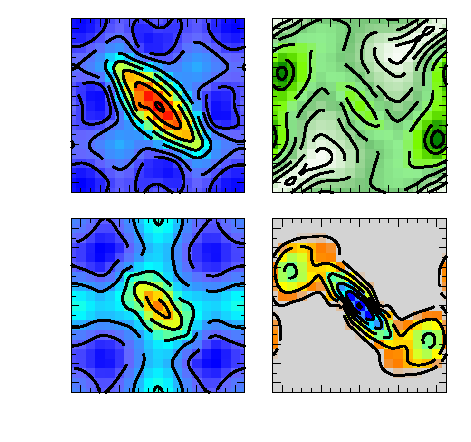
\includegraphics[width={453.00bp},height={453.00bp}]{chapters/results/image/Q0_maps}}%
    \gplfronttext
  \end{picture}%
\endgroup

		\end{column}
		\begin{column}[c]{0.3\textwidth}
			\centering
			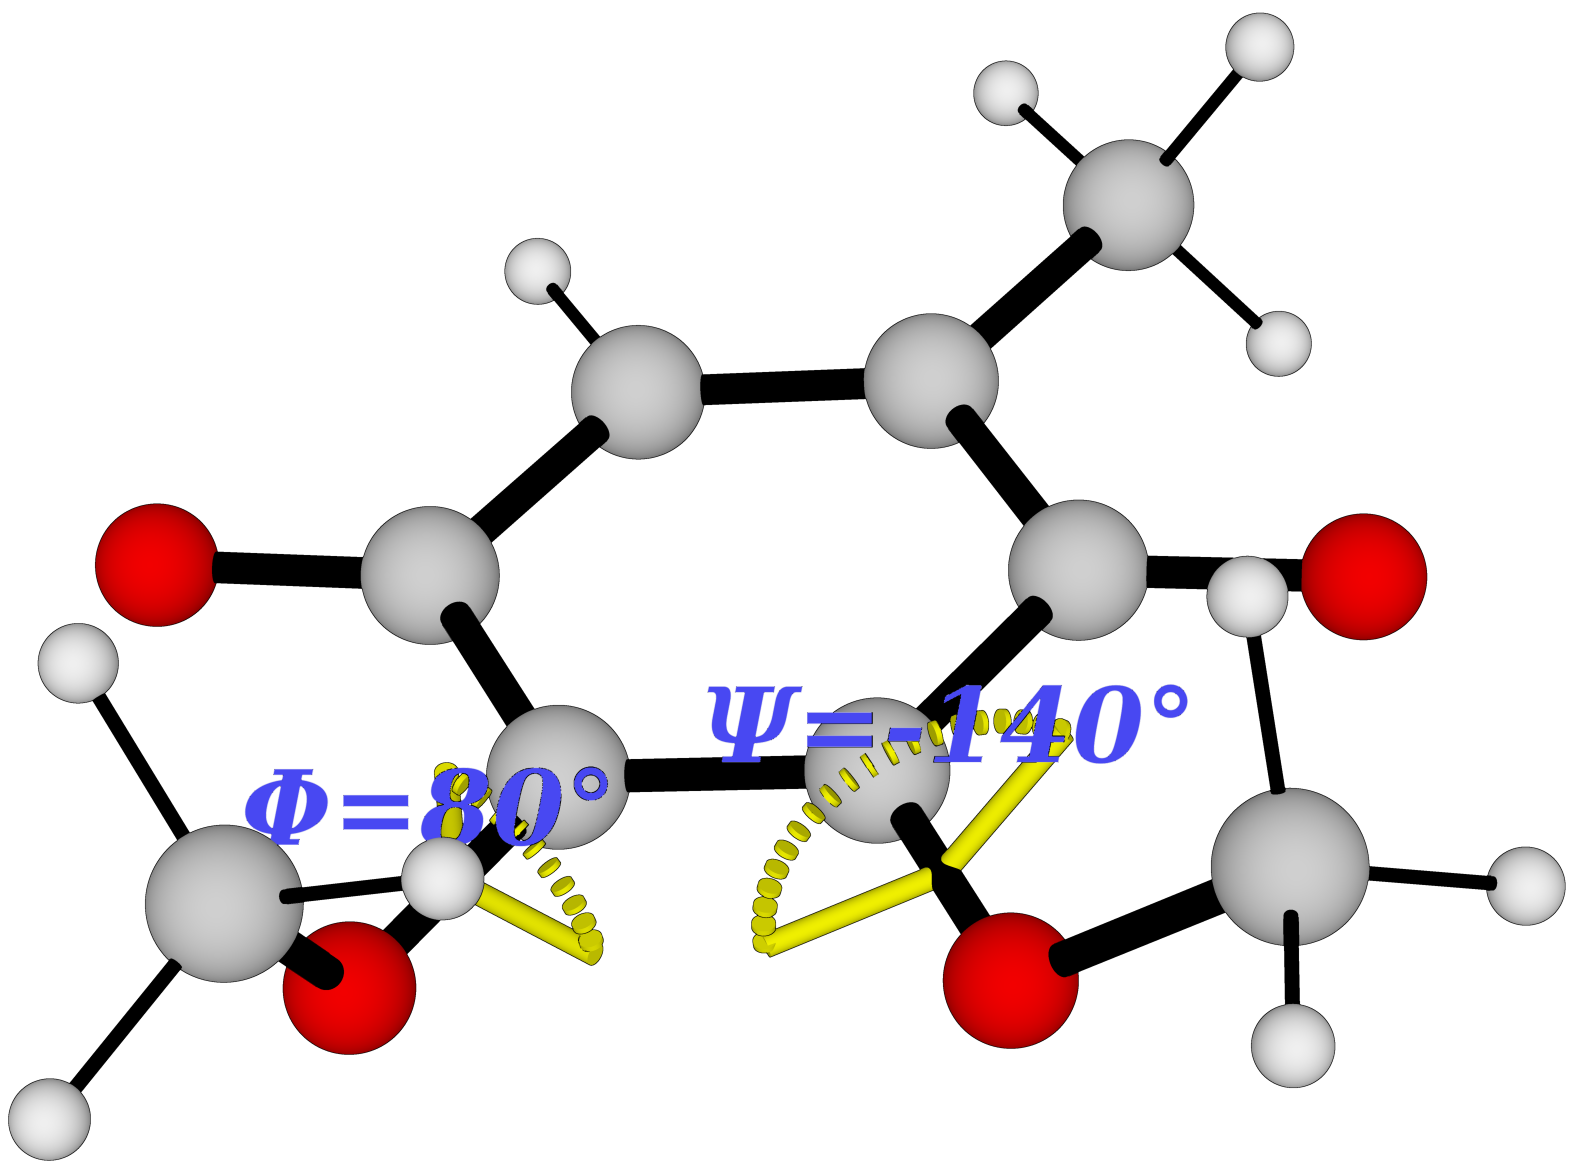
\includegraphics[width=\textwidth]{Figs/dihedrals.png}
			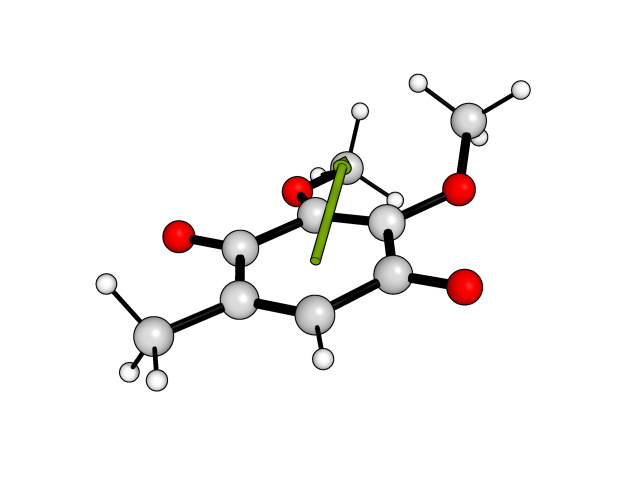
\includegraphics[width=0.6\textwidth]{Figs/Q0_181.png}
			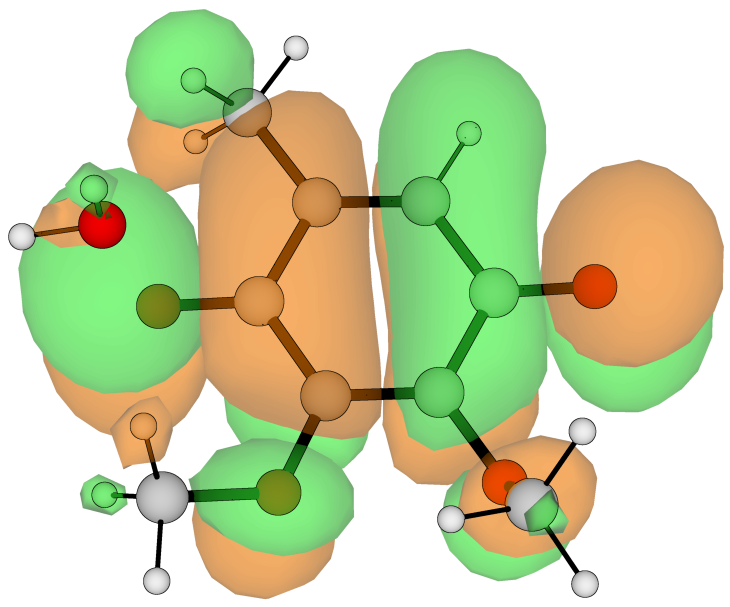
\includegraphics[width=0.6\textwidth]{Figs/Q0_H2O_VBS.png}
			\vspace{30pt}
		\end{column}
	\end{columns}
	\Put(310,190){\fontsize{6}{4}\selectfont\text{DBA}}
	\Put(310,70){\fontsize{6}{4}\selectfont\text{VBA}}
\end{frame}

\begin{frame}
	\frametitle{DBA populations}\large
	Two distinct types of dipole-bound anions (DBA) are observed.
		\begin{columns}
		\begin{column}[c]{0.5\textwidth}
			\footnotesize
			% GNUPLOT: LaTeX picture with Postscript
\begingroup
  \makeatletter
  \providecommand\color[2][]{%
    \GenericError{(gnuplot) \space\space\space\@spaces}{%
      Package color not loaded in conjunction with
      terminal option `colourtext'%
    }{See the gnuplot documentation for explanation.%
    }{Either use 'blacktext' in gnuplot or load the package
      color.sty in LaTeX.}%
    \renewcommand\color[2][]{}%
  }%
  \providecommand\includegraphics[2][]{%
    \GenericError{(gnuplot) \space\space\space\@spaces}{%
      Package graphicx or graphics not loaded%
    }{See the gnuplot documentation for explanation.%
    }{The gnuplot epslatex terminal needs graphicx.sty or graphics.sty.}%
    \renewcommand\includegraphics[2][]{}%
  }%
  \providecommand\rotatebox[2]{#2}%
  \@ifundefined{ifGPcolor}{%
    \newif\ifGPcolor
    \GPcolortrue
  }{}%
  \@ifundefined{ifGPblacktext}{%
    \newif\ifGPblacktext
    \GPblacktexttrue
  }{}%
  % define a \g@addto@macro without @ in the name:
  \let\gplgaddtomacro\g@addto@macro
  % define empty templates for all commands taking text:
  \gdef\gplbacktext{}%
  \gdef\gplfronttext{}%
  \makeatother
  \ifGPblacktext
    % no textcolor at all
    \def\colorrgb#1{}%
    \def\colorgray#1{}%
  \else
    % gray or color?
    \ifGPcolor
      \def\colorrgb#1{\color[rgb]{#1}}%
      \def\colorgray#1{\color[gray]{#1}}%
      \expandafter\def\csname LTw\endcsname{\color{white}}%
      \expandafter\def\csname LTb\endcsname{\color{black}}%
      \expandafter\def\csname LTa\endcsname{\color{black}}%
      \expandafter\def\csname LT0\endcsname{\color[rgb]{1,0,0}}%
      \expandafter\def\csname LT1\endcsname{\color[rgb]{0,1,0}}%
      \expandafter\def\csname LT2\endcsname{\color[rgb]{0,0,1}}%
      \expandafter\def\csname LT3\endcsname{\color[rgb]{1,0,1}}%
      \expandafter\def\csname LT4\endcsname{\color[rgb]{0,1,1}}%
      \expandafter\def\csname LT5\endcsname{\color[rgb]{1,1,0}}%
      \expandafter\def\csname LT6\endcsname{\color[rgb]{0,0,0}}%
      \expandafter\def\csname LT7\endcsname{\color[rgb]{1,0.3,0}}%
      \expandafter\def\csname LT8\endcsname{\color[rgb]{0.5,0.5,0.5}}%
    \else
      % gray
      \def\colorrgb#1{\color{black}}%
      \def\colorgray#1{\color[gray]{#1}}%
      \expandafter\def\csname LTw\endcsname{\color{white}}%
      \expandafter\def\csname LTb\endcsname{\color{black}}%
      \expandafter\def\csname LTa\endcsname{\color{black}}%
      \expandafter\def\csname LT0\endcsname{\color{black}}%
      \expandafter\def\csname LT1\endcsname{\color{black}}%
      \expandafter\def\csname LT2\endcsname{\color{black}}%
      \expandafter\def\csname LT3\endcsname{\color{black}}%
      \expandafter\def\csname LT4\endcsname{\color{black}}%
      \expandafter\def\csname LT5\endcsname{\color{black}}%
      \expandafter\def\csname LT6\endcsname{\color{black}}%
      \expandafter\def\csname LT7\endcsname{\color{black}}%
      \expandafter\def\csname LT8\endcsname{\color{black}}%
    \fi
  \fi
    \setlength{\unitlength}{0.0500bp}%
    \ifx\gptboxheight\undefined%
      \newlength{\gptboxheight}%
      \newlength{\gptboxwidth}%
      \newsavebox{\gptboxtext}%
    \fi%
    \setlength{\fboxrule}{0.5pt}%
    \setlength{\fboxsep}{1pt}%
    \definecolor{tbcol}{rgb}{1,1,1}%
\begin{picture}(6500.00,2540.00)%
    \gplgaddtomacro\gplbacktext{%
      \csname LTb\endcsname%%
      \put(420,453){\makebox(0,0)[r]{\strut{}$0$}}%
      \csname LTb\endcsname%%
      \put(420,729){\makebox(0,0)[r]{\strut{}$2$}}%
      \csname LTb\endcsname%%
      \put(420,1004){\makebox(0,0)[r]{\strut{}$4$}}%
      \csname LTb\endcsname%%
      \put(420,1280){\makebox(0,0)[r]{\strut{}$6$}}%
      \csname LTb\endcsname%%
      \put(420,1555){\makebox(0,0)[r]{\strut{}$8$}}%
      \csname LTb\endcsname%%
      \put(420,1831){\makebox(0,0)[r]{\strut{}$10$}}%
      \csname LTb\endcsname%%
      \put(420,2106){\makebox(0,0)[r]{\strut{}$12$}}%
      \csname LTb\endcsname%%
      \put(420,2382){\makebox(0,0)[r]{\strut{}$14$}}%
      \csname LTb\endcsname%%
      \put(518,277){\makebox(0,0){\strut{}$1.5$}}%
      \csname LTb\endcsname%%
      \put(1181,277){\makebox(0,0){\strut{}$2$}}%
      \csname LTb\endcsname%%
      \put(1843,277){\makebox(0,0){\strut{}$2.5$}}%
      \csname LTb\endcsname%%
      \put(2506,277){\makebox(0,0){\strut{}$3$}}%
      \csname LTb\endcsname%%
      \put(3169,277){\makebox(0,0){\strut{}$3.5$}}%
      \csname LTb\endcsname%%
      \put(810,2354){\makebox(0,0){\strut{}Q0}}%
    }%
    \gplgaddtomacro\gplfronttext{%
      \csname LTb\endcsname%%
      \put(2913,2297){\makebox(0,0)[r]{\strut{}Region A}}%
      \csname LTb\endcsname%%
      \put(2913,2122){\makebox(0,0)[r]{\strut{}Region B}}%
      \csname LTb\endcsname%%
      \put(63,1486){\rotatebox{-270.00}{\makebox(0,0){\strut{}DBS Binding Energy (meV)}}}%
      \csname LTb\endcsname%%
      \put(1976,13){\makebox(0,0){\strut{}Dipole Strength (Debye)}}%
    }%
    \gplgaddtomacro\gplbacktext{%
      \csname LTb\endcsname%%
      \put(3466,453){\makebox(0,0)[r]{\strut{}}}%
      \csname LTb\endcsname%%
      \put(3466,729){\makebox(0,0)[r]{\strut{}}}%
      \csname LTb\endcsname%%
      \put(3466,1004){\makebox(0,0)[r]{\strut{}}}%
      \csname LTb\endcsname%%
      \put(3466,1280){\makebox(0,0)[r]{\strut{}}}%
      \csname LTb\endcsname%%
      \put(3466,1555){\makebox(0,0)[r]{\strut{}}}%
      \csname LTb\endcsname%%
      \put(3466,1831){\makebox(0,0)[r]{\strut{}}}%
      \csname LTb\endcsname%%
      \put(3466,2106){\makebox(0,0)[r]{\strut{}}}%
      \csname LTb\endcsname%%
      \put(3466,2382){\makebox(0,0)[r]{\strut{}}}%
      \csname LTb\endcsname%%
      \put(3564,277){\makebox(0,0){\strut{}$1.5$}}%
      \csname LTb\endcsname%%
      \put(4226,277){\makebox(0,0){\strut{}$2$}}%
      \csname LTb\endcsname%%
      \put(4889,277){\makebox(0,0){\strut{}$2.5$}}%
      \csname LTb\endcsname%%
      \put(5552,277){\makebox(0,0){\strut{}$3$}}%
      \csname LTb\endcsname%%
      \put(6214,277){\makebox(0,0){\strut{}$3.5$}}%
      \csname LTb\endcsname%%
      \put(3855,2354){\makebox(0,0){\strut{}Q1}}%
    }%
    \gplgaddtomacro\gplfronttext{%
      \csname LTb\endcsname%%
      \put(5959,2385){\makebox(0,0)[r]{\strut{}Region A}}%
      \csname LTb\endcsname%%
      \put(5959,2209){\makebox(0,0)[r]{\strut{}Region B}}%
      \csname LTb\endcsname%%
      \put(5959,2034){\makebox(0,0)[r]{\strut{}Region C}}%
      \csname LTb\endcsname%%
      \put(5021,13){\makebox(0,0){\strut{}Dipole Strength (Debye)}}%
    }%
    \gplbacktext
    \put(0,0){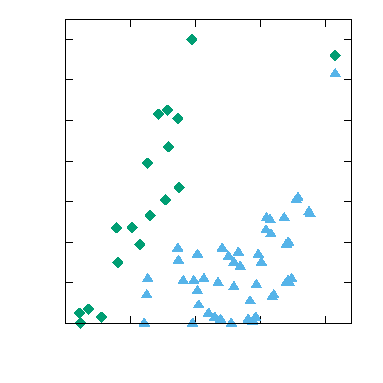
\includegraphics[width={325.00bp},height={127.00bp}]{Figs/DvsDBS}}%
    \gplfronttext
  \end{picture}%
\endgroup

		\end{column}
		\begin{column}[c]{0.5\textwidth}
			\centering
			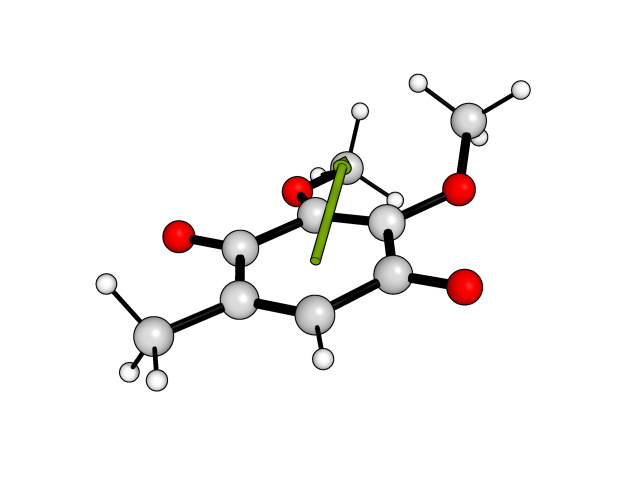
\includegraphics[width=0.45\textwidth]{Figs/Q0_181.png}Region A\\
			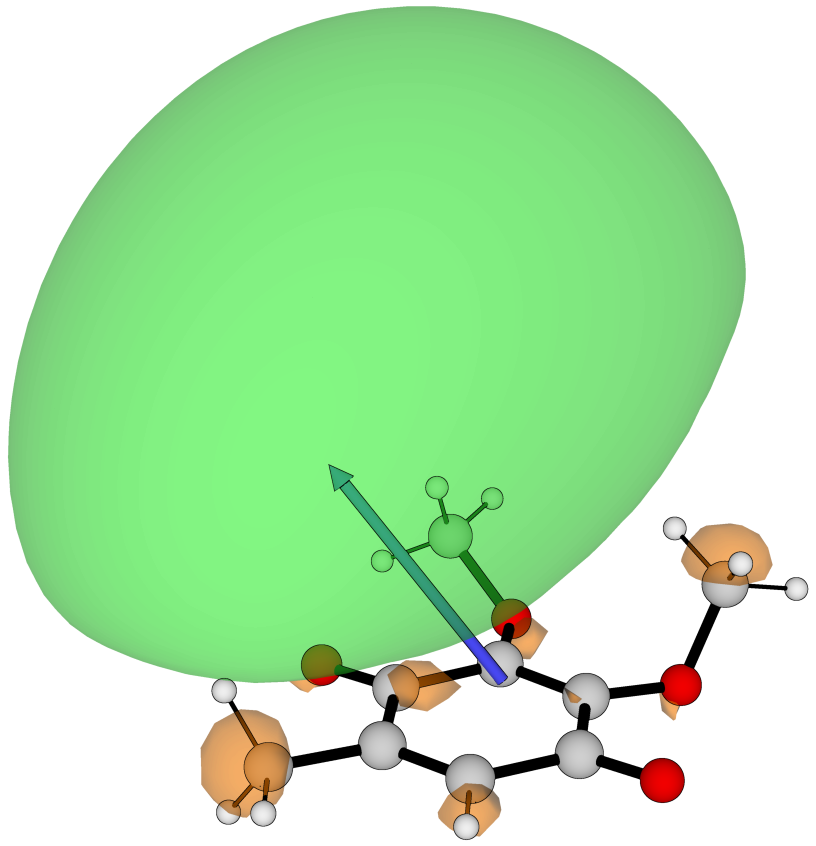
\includegraphics[width=0.45\textwidth]{Figs/Q0_52.png} Region B\\
			\vspace{30pt}
		\end{column}
	\end{columns}	
\end{frame}

\begin{frame}{\huge A simple cluster model}\large
	A directed interaction with small molecules\\ strongly stabilises the DBA.
	\vspace{10pt}
	\Put(100,3){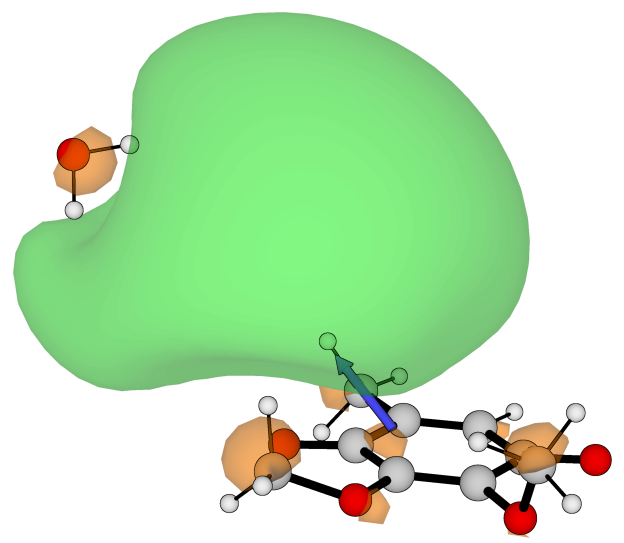
\includegraphics[width=0.3\textwidth]{Figs/Q0_H2O_H.png}}
	% GNUPLOT: LaTeX picture with Postscript
\begingroup
  \makeatletter
  \providecommand\color[2][]{%
    \GenericError{(gnuplot) \space\space\space\@spaces}{%
      Package color not loaded in conjunction with
      terminal option `colourtext'%
    }{See the gnuplot documentation for explanation.%
    }{Either use 'blacktext' in gnuplot or load the package
      color.sty in LaTeX.}%
    \renewcommand\color[2][]{}%
  }%
  \providecommand\includegraphics[2][]{%
    \GenericError{(gnuplot) \space\space\space\@spaces}{%
      Package graphicx or graphics not loaded%
    }{See the gnuplot documentation for explanation.%
    }{The gnuplot epslatex terminal needs graphicx.sty or graphics.sty.}%
    \renewcommand\includegraphics[2][]{}%
  }%
  \providecommand\rotatebox[2]{#2}%
  \@ifundefined{ifGPcolor}{%
    \newif\ifGPcolor
    \GPcolortrue
  }{}%
  \@ifundefined{ifGPblacktext}{%
    \newif\ifGPblacktext
    \GPblacktexttrue
  }{}%
  % define a \g@addto@macro without @ in the name:
  \let\gplgaddtomacro\g@addto@macro
  % define empty templates for all commands taking text:
  \gdef\gplbacktext{}%
  \gdef\gplfronttext{}%
  \makeatother
  \ifGPblacktext
    % no textcolor at all
    \def\colorrgb#1{}%
    \def\colorgray#1{}%
  \else
    % gray or color?
    \ifGPcolor
      \def\colorrgb#1{\color[rgb]{#1}}%
      \def\colorgray#1{\color[gray]{#1}}%
      \expandafter\def\csname LTw\endcsname{\color{white}}%
      \expandafter\def\csname LTb\endcsname{\color{black}}%
      \expandafter\def\csname LTa\endcsname{\color{black}}%
      \expandafter\def\csname LT0\endcsname{\color[rgb]{1,0,0}}%
      \expandafter\def\csname LT1\endcsname{\color[rgb]{0,1,0}}%
      \expandafter\def\csname LT2\endcsname{\color[rgb]{0,0,1}}%
      \expandafter\def\csname LT3\endcsname{\color[rgb]{1,0,1}}%
      \expandafter\def\csname LT4\endcsname{\color[rgb]{0,1,1}}%
      \expandafter\def\csname LT5\endcsname{\color[rgb]{1,1,0}}%
      \expandafter\def\csname LT6\endcsname{\color[rgb]{0,0,0}}%
      \expandafter\def\csname LT7\endcsname{\color[rgb]{1,0.3,0}}%
      \expandafter\def\csname LT8\endcsname{\color[rgb]{0.5,0.5,0.5}}%
    \else
      % gray
      \def\colorrgb#1{\color{black}}%
      \def\colorgray#1{\color[gray]{#1}}%
      \expandafter\def\csname LTw\endcsname{\color{white}}%
      \expandafter\def\csname LTb\endcsname{\color{black}}%
      \expandafter\def\csname LTa\endcsname{\color{black}}%
      \expandafter\def\csname LT0\endcsname{\color{black}}%
      \expandafter\def\csname LT1\endcsname{\color{black}}%
      \expandafter\def\csname LT2\endcsname{\color{black}}%
      \expandafter\def\csname LT3\endcsname{\color{black}}%
      \expandafter\def\csname LT4\endcsname{\color{black}}%
      \expandafter\def\csname LT5\endcsname{\color{black}}%
      \expandafter\def\csname LT6\endcsname{\color{black}}%
      \expandafter\def\csname LT7\endcsname{\color{black}}%
      \expandafter\def\csname LT8\endcsname{\color{black}}%
    \fi
  \fi
    \setlength{\unitlength}{0.0500bp}%
    \ifx\gptboxheight\undefined%
      \newlength{\gptboxheight}%
      \newlength{\gptboxwidth}%
      \newsavebox{\gptboxtext}%
    \fi%
    \setlength{\fboxrule}{0.5pt}%
    \setlength{\fboxsep}{1pt}%
    \definecolor{tbcol}{rgb}{1,1,1}%
\begin{picture}(6980.00,3480.00)%
    \gplgaddtomacro\gplbacktext{%
      \csname LTb\endcsname%%
      \put(598,2006){\makebox(0,0)[r]{\strut{}-80}}%
      \csname LTb\endcsname%%
      \put(598,2332){\makebox(0,0)[r]{\strut{}-60}}%
      \csname LTb\endcsname%%
      \put(598,2658){\makebox(0,0)[r]{\strut{}-40}}%
      \csname LTb\endcsname%%
      \put(598,2983){\makebox(0,0)[r]{\strut{}-20}}%
      \csname LTb\endcsname%%
      \put(598,3309){\makebox(0,0)[r]{\strut{}0}}%
      \csname LTb\endcsname%%
      \put(1149,1830){\makebox(0,0){\strut{}}}%
      \csname LTb\endcsname%%
      \put(2283,1830){\makebox(0,0){\strut{}}}%
      \csname LTb\endcsname%%
      \put(3418,1830){\makebox(0,0){\strut{}}}%
      \csname LTb\endcsname%%
      \put(4552,1830){\makebox(0,0){\strut{}}}%
      \csname LTb\endcsname%%
      \put(5686,1830){\makebox(0,0){\strut{}}}%
      \csname LTb\endcsname%%
      \put(6820,1830){\makebox(0,0){\strut{}}}%
      \csname LTb\endcsname%%
      \put(3758,2145){\makebox(0,0){\strut{}DBS Parallel}}%
    }%
    \gplgaddtomacro\gplfronttext{%
      \csname LTb\endcsname%%
      \put(45,2698){\rotatebox{-270.00}{\makebox(0,0){\strut{}Energy (meV)}}}%
    }%
    \gplgaddtomacro\gplbacktext{%
      \csname LTb\endcsname%%
      \put(598,519){\makebox(0,0)[r]{\strut{}-2.0}}%
      \csname LTb\endcsname%%
      \put(598,980){\makebox(0,0)[r]{\strut{}-1.8}}%
      \csname LTb\endcsname%%
      \put(598,1441){\makebox(0,0)[r]{\strut{}-1.6}}%
      \csname LTb\endcsname%%
      \put(598,1902){\makebox(0,0)[r]{\strut{}-1.4}}%
      \csname LTb\endcsname%%
      \put(1149,343){\makebox(0,0){\strut{}$5$}}%
      \csname LTb\endcsname%%
      \put(2283,343){\makebox(0,0){\strut{}$10$}}%
      \csname LTb\endcsname%%
      \put(3418,343){\makebox(0,0){\strut{}$15$}}%
      \csname LTb\endcsname%%
      \put(4552,343){\makebox(0,0){\strut{}$20$}}%
      \csname LTb\endcsname%%
      \put(5686,343){\makebox(0,0){\strut{}$25$}}%
      \csname LTb\endcsname%%
      \put(6820,343){\makebox(0,0){\strut{}$30$}}%
      \csname LTb\endcsname%%
      \put(3758,657){\makebox(0,0){\strut{}VBS Parallel}}%
    }%
    \gplgaddtomacro\gplfronttext{%
      \csname LTb\endcsname%%
      \put(45,1210){\rotatebox{-270.00}{\makebox(0,0){\strut{}Energy (eV)}}}%
      \csname LTb\endcsname%%
      \put(3758,79){\makebox(0,0){\strut{}Distance (\AA)}}%
    }%
    \gplbacktext
    \put(0,0){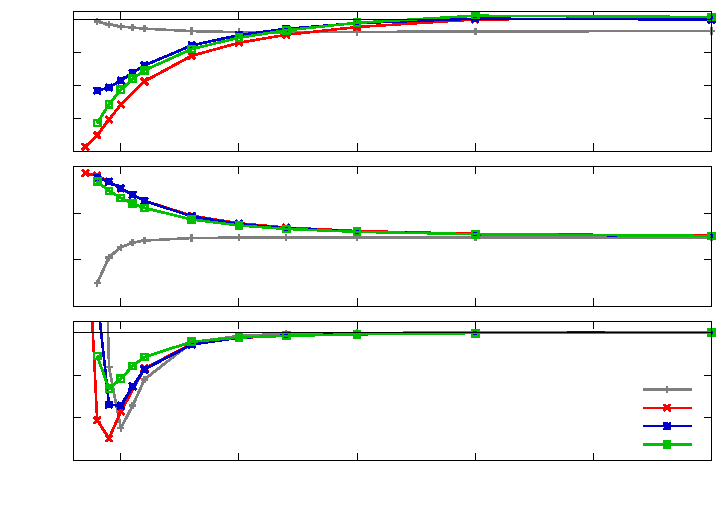
\includegraphics[width={349.00bp},height={174.00bp}]{scan_X}}%
    \gplfronttext
  \end{picture}%
\endgroup

\end{frame}

\begin{frame}{\huge Conclusions}\large
	\begin{itemize}
		\item Distinction between valence and Non-valence anions.
		\item Dipole Strength is correlated with DBA energy for similar chemical contexts.
		\item Surrounding molecules can have a big effect on the states.
	\end{itemize}
	\centering
	\vspace{40pt}
	\Huge \textcolor{kul-blue}{\textbf{Thanks for your attention!}}
\end{frame}

\begin{frame}{\huge Acknowledgements}\large
	\centering
	\begin{columns}
		\begin{column}[c]{0.7\textwidth}
			\centering
			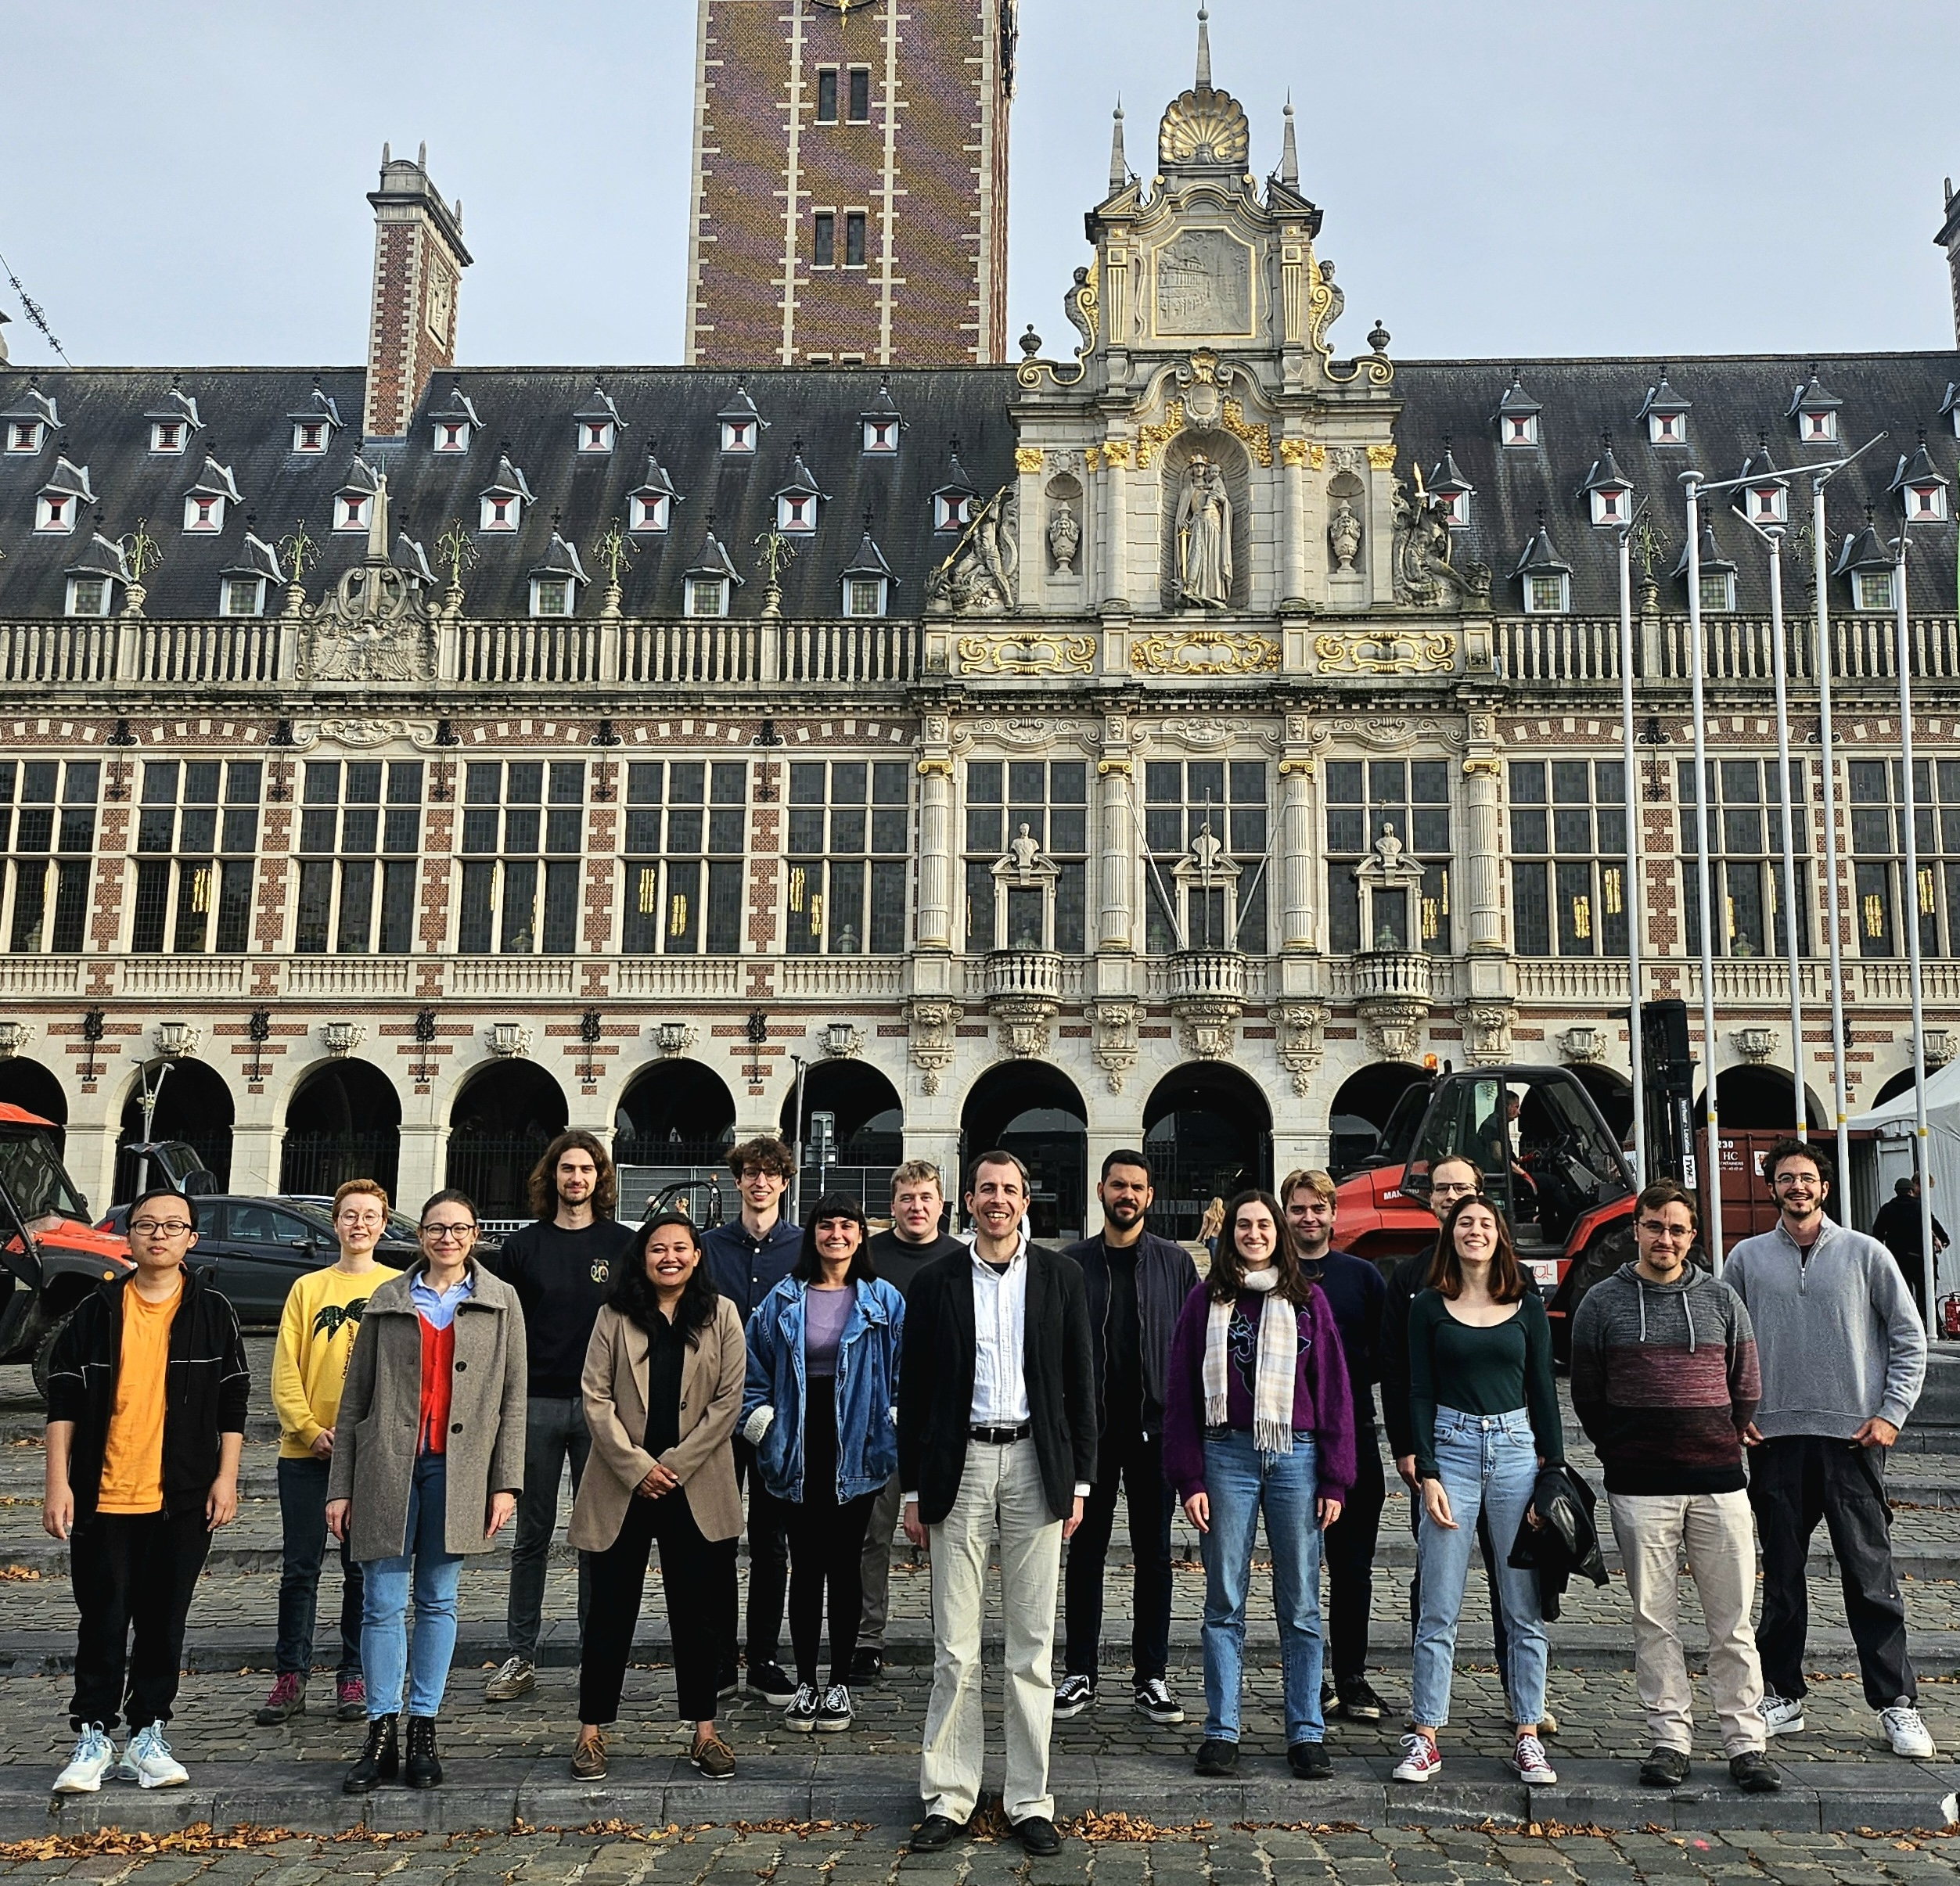
\includegraphics[width=\textwidth]{Figs/TJ.jpeg}
		\end{column}
		\begin{column}[c]{0.3\textwidth}
			\centering
			
\includegraphics[width=\textwidth]{Figs/VSC-Combilogo.png}\\\vfill
			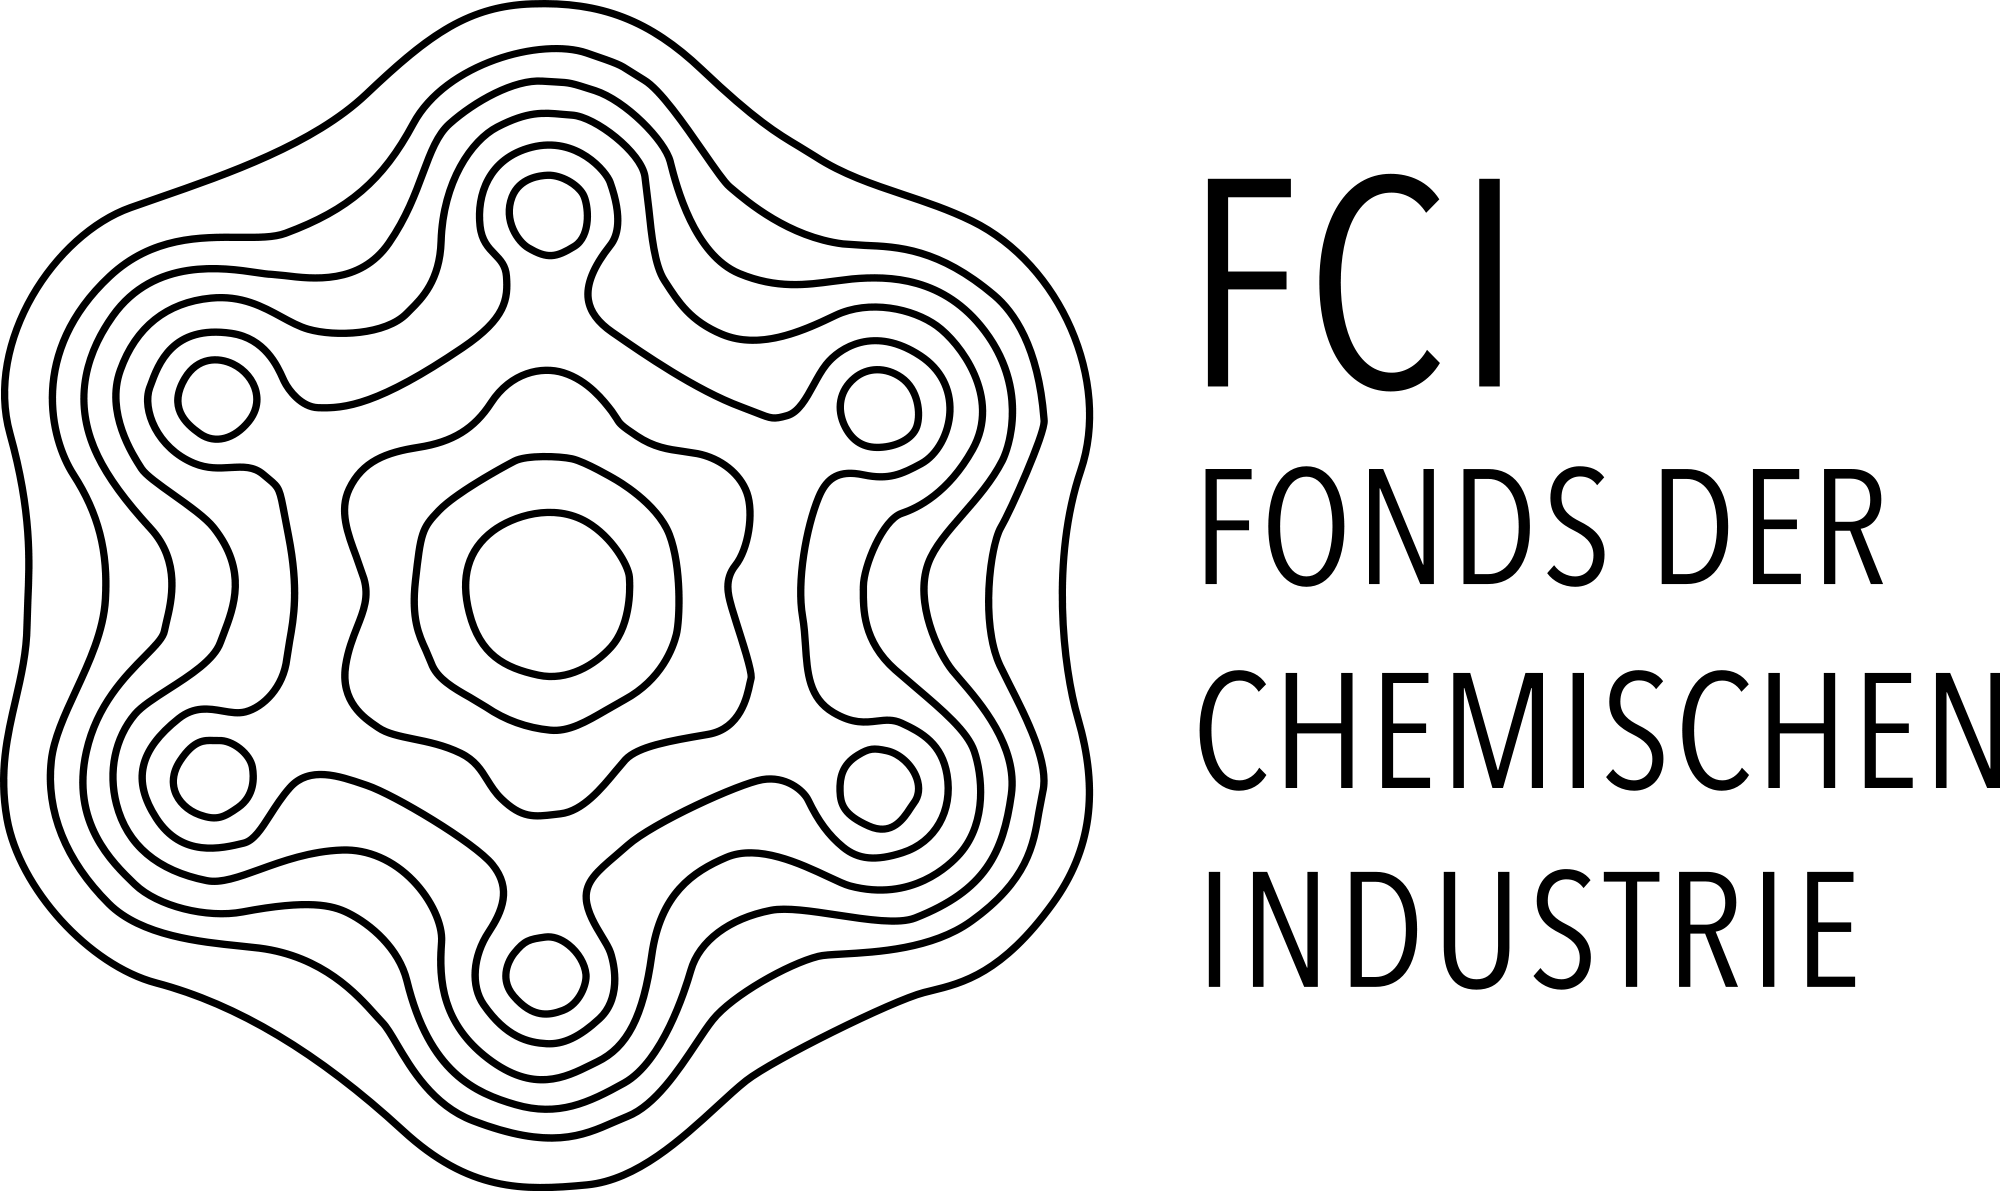
\includegraphics[width=0.6\textwidth]{Figs/FCI.png}\\\vfill
			
\includegraphics[width=0.7\textwidth]{Figs/erc.png}\\\vfill
			
\includegraphics[width=0.45\textwidth]{Figs/La-Caixa.png}\\\vfill
			
\includegraphics[width=\textwidth]{Figs/QCLogo.png}\\\vfill
		\end{column}
	\end{columns}

	\vspace{3pt}
\end{frame}

\iffalse
\begin{frame}{\huge Basis set convergence}\large
	Basis size and \# of extra diffuse functions effect on dipole bound states\\
	\begin{table}[h!]
		\centering
		\footnotesize
		\begin{tabular}{lccccc}
		 & \multicolumn{3}{c}{RI-CC2} & \multicolumn{2}{c}{RI-CCSD} \\
		\cmidrule(lr){2-4} \cmidrule(lr){5-6}
		 & pVDZ+6s3p & pVTZ+6s3p & pQDZ+6s3p & pVDZ+6s3p & pVTZ+6s3p \\
		\midrule
		acetaldehide & 4.6 & 3.2 & 3.2 & 4.6 & 3.1 \\
		acetone & 0.3 & -1.3 & -0.9 & 0.5 & -0.9 \\
		acetonitrile & -18.2 & -19.9 & -20.3 & -17.1 & -18.4 \\
		benzaldehide & 7.4 & 8.9 & 9.1 & 3.4 & 4.6 \\
		dimethylformamide & 13.2 & 14.1 & 14.4 & 13.3 & 13.7 \\
		dmso & 14.8 & 15.4 & 15.5 & 14.7 & 14.9 \\
		formamide & -16.1 & -16.2 & -17.0 & -15.1 & -15.9 \\
		methylisocyanide & -9.5 & -10.0 & -10.1 & -8.8 & -9.0 \\
		nitrobenzene & -32.5 & -34.8 & - & -28.0 & -25.9 \\
		nitromethane & -13.0 & -14.2 & -14.7 & -12.9 & -13.7 \\
		nitrosobenzene & -9.9 & -11.4 & - & -5.1 & -6.0 \\
		phenylisocyanide & -15.2 & -16.3 & -16.7 & -9.0 & -9.2 \\
		pyridazine & -26.0 & -26.3 & -26.7 & -18.6 & -19.1 \\
		vinylene carbonate& -26.4 & -27.2 & -27.7 & -25.1 & -25.5 \\
		\midrule
		\textbf{MAE} & \textbf{2.3} & \textbf{2.8} & \textbf{2.4} & \textbf{0.8} & \textbf{-} \\
		\bottomrule
		\end{tabular}
	\end{table}
\end{frame}

\begin{frame}{\huge Computational methods}\large
	\vspace{5pt}
	\begin{itemize}
		\item Optimizations performed at TPSS+D3BJ/ma-def2-TZVP
		EA calculated at the RI-EOM-EA-CC2 using the neutral ground state as CC reference state
		\item aug-cc-pVTZ basis further augmented by 3 s-shells on Hydrogen atoms and 6 s- and 3 p-shells on all non-hydrogen atoms
	\end{itemize}
	\vspace{35pt}
	\centering
	
\includegraphics[width=0.5\textwidth]{Figs/QCLogo.png}
\end{frame}

% --- New Slide: How do we treat electronic structure theoretically? ---

\begin{frame}{\huge Theoretical treatment of electronic structure}\large
    \vspace{5pt}
    \begin{itemize}
        \item Quantum chemistry describes molecules by solving the Schrödinger equation for electrons and nuclei.
        \item Approximations are needed for all but the smallest systems.
        \item \textbf{Key concepts:}
        \begin{itemize}
            \item Molecular orbitals
            \item Electron correlation
            \item Basis sets
        \end{itemize}
    \end{itemize}
    \vspace{5pt}
    \centering
    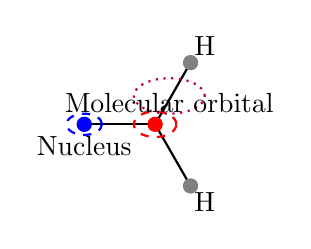
\begin{tikzpicture}[scale=0.9]
        % Draw molecule
        \draw[thick] (0,0) -- (1,0);
        \draw[thick] (1,0) -- (1.5,0.87);
        \draw[thick] (1,0) -- (1.5,-0.87);
        \filldraw[blue] (0,0) circle (0.1);
        \filldraw[red] (1,0) circle (0.1);
        \filldraw[gray] (1.5,0.87) circle (0.1);
        \filldraw[gray] (1.5,-0.87) circle (0.1);
        % Draw orbitals
        \draw[thick, dashed, blue] (0,0) ellipse (0.25 and 0.15);
        \draw[thick, dashed, red] (1,0) ellipse (0.3 and 0.18);
        % Electron cloud
        \draw[thick, dotted, purple] (1.2,0.4) ellipse (0.5 and 0.25);
        % Labels
        \node at (0,-0.3) {Nucleus};
        \node at (1.7,1.1) {H};
        \node at (1.7,-1.1) {H};
        \node at (1.2,0.3) {Molecular orbital};
    \end{tikzpicture}
\end{frame}

\begin{frame}{\huge CC2}\large
	Second-order approximate coupled-cluster singles and doubles (CC2) method is obtained from a perturbative analysis of the CCSD model
	\vspace{5pt}
	\begin{itemize}
		\item Lowers computational scaling from CCSD 
		\item Allows treatment of “big” molecules: $>$ 25 heavy atoms
	\end{itemize}
	\centering
	\vspace{30pt}
	\begin{table}
		\centering
		\begin{tabular}{lcc}\toprule
		\textbf{Method} & \textbf{Scaling} & \textbf{Memory}\\\midrule
		CCSD & $O(N^6)$ & $O(N^{4})^*$\\
		CC2 & $O(N^5)$ & $O(N^{4})^*$\\\bottomrule
		\multicolumn{3}{l}{\small $^*\,O(N^3)$ with RI approximation.}
		\end{tabular}
	\end{table}
\end{frame}

\begin{frame}{\huge Quantum chemical methods}\large
	The time independent Schrödinger equation is approximatelly solved to describe the electronic structure of molecules:
	\begin{equation*}
		\hat{H} \Psi = E \Psi
	\end{equation*}
	We construct the wavefunction $\Psi$ as a combination of molecular orbitals (MOs):
	\begin{equation*}
		\Psi = \sum_{i} c_i \phi_i
	\end{equation*}
\end{frame}
\fi

\end{document}
